\documentclass[journal]{IEEEtran}
\usepackage{graphicx}
\usepackage{booktabs}
\usepackage{array}
\usepackage{url}
\usepackage{cite}
\usepackage{amsmath,amssymb}
\usepackage{balance}
\def\IEEEbibitemsep{0pt plus .3pt}
\begin{document}

\title{Machine learning in battery management systems: a structured scoping review and classification of 103 peer-reviewed studies, 2019--2026}

\author{Hussain~Touhid~Siddiquee,~Syeda~Salsabil~Islam~Ariya,~and~Jasimul~Islam~Chowdhury%
\thanks{Manuscript received September 2026. (Corresponding author: Hussain Touhid Siddiquee.)}%
\thanks{The authors are with Leading University, Sylhet, Bangladesh. The classified corpus,
the conference sensitivity set, and the complete analysis pipeline are publicly available at
\texttt{github.com/touhidsiddiqueeraj-bit}.}}

\markboth{IEEE Transactions Submission, September 2026}{Siddiquee et al.: Machine Learning in Battery Management Systems}

\maketitle

\begin{abstract}
Machine learning (ML) has moved from a promising addition to battery research to a load-bearing component of modern battery management systems (BMS), yet the validation practices behind the literature's accuracy claims have never been systematically measured. This paper presents a structured scoping review of 103 peer-reviewed journal articles (2019--2026) --- assembled from a Crossref-verified pool and classified uniformly by management function, method family, chemistry, data source, and validation practice --- supported by a 14-paper conference sensitivity set. The bibliometric analysis reveals a clear evolution: classical shallow learners dominated 2019--2021, deep sequence models rose sharply in 2022--2023, physics-informed and hybrid model--data approaches became one of the fastest-growing families (24 of 103 papers), and the first large-language-model-based management studies appear in 2025--2026. Health estimation and prognostics remain the largest application cluster (35 papers). Three structural weaknesses persist. Only 9 of 103 studies demonstrate online or fleet-level operation, while 17 rely on within-cell or k-fold splits that overstate generalization; benchmark reliance is narrow, with 23 papers resting on three public datasets; and the laboratory-to-field gap remains the field's defining challenge. The review's sharpest finding is that physics-informed architectures, often assumed to improve reliability by construction, are validated less rigorously than purely data-driven peers (54\% versus 73\% strong-protocol share): physics priors reduce data demand but do not substitute for rigorous out-of-distribution testing. The paper closes with a conference-path sensitivity analysis, a safety taxonomy for foundation-model components, and a twelve-item reporting checklist for future machine-learning BMS studies.
\end{abstract}

\begin{IEEEkeywords}
machine learning, battery management systems, lithium-ion batteries, state of charge, state of health, remaining useful life, deep learning, physics-informed neural networks, transfer learning, battery safety
\end{IEEEkeywords}

\section{Introduction}

\subsection{The battery management problem}

Lithium-ion batteries now anchor three converging transitions --- electrified road transport, renewable-heavy stationary storage, and the electrification of aerospace and marine systems --- and in each the battery is an actively managed asset whose usable capacity, lifetime, and safety depend on real-time operating decisions. The battery management system (BMS) is the embedded cyber-physical layer that makes those decisions --- sensing, state estimation, protection, balancing, and charging negotiation \cite{r1}. The difficulty stems from the fact that the quantities that matter most --- state of charge (SOC), state of health (SOH), internal temperature, and the onset of degradation or fault mechanisms --- are not directly measurable and must be inferred from noisy, partially observable terminal measurements under widely varying conditions. Model-based approaches built on equivalent-circuit or electrochemical models face a persistent fidelity-versus-tractability trade-off, and their parameters drift as cells age \cite{r2}. It is in this inference-and-decision layer that machine learning has made its most forceful entry, and nowhere with more at stake than in transportation: electric-vehicle packs face automotive safety expectations (UN GTR 20, GB 38031, ISO 26262) that make estimation and prognosis safety-relevant functions, ten of the corpus studies are demonstrated on real vehicle or fleet data, and the field's newest direction --- vehicle-cloud orchestration --- is itself automotive.

Machine learning entered battery management through estimation on hand-engineered features. Two studies then reset expectations. Severson and colleagues predicted the entire cycle life of lithium-ion cells with a median test error near 9\% from the first hundred cycles alone, on a public dataset of 124 cells \cite{r3}. Attia and colleagues demonstrated closed-loop Bayesian optimization of fast-charging protocols in 2.5 months rather than 18 months of manual experimentation \cite{r4}. The five years that followed produced applications across every BMS function: recurrent and convolutional networks for SOC and SOH \cite{r5}\cite{r6}, graph and transformer architectures for prognostics \cite{r7}\cite{r8}, physics-informed neural networks embedding electrochemical and thermal priors \cite{r9}\cite{r10}, transfer learning across chemistries and vehicles \cite{r11}\cite{r12}, reinforcement learning agents \cite{r13}, and, most recently, large language model (LLM) agents for fleet-scale risk analysis and vehicle-cloud management \cite{r14}\cite{r15}.

\subsection{Existing reviews and the literature gap}

The review literature has grown alongside the applications but is fragmented along the same axes as the primary studies: function-specific reviews cover SOC estimation \cite{r16}\cite{r17}, SOH estimation \cite{r18}, and prognostics \cite{r19}; method-specific reviews follow deep-learning state estimation \cite{r20}, physics-informed impedance diagnostics \cite{r21}, or interpretable prognosis \cite{r22}; and domain reviews examine fault diagnosis \cite{r23}\cite{r24} and thermal management \cite{r25}, alongside broader degradation-method surveys \cite{r26}. What is missing is a cross-functional account of the field's trajectory: which method families are used for which tasks, on which data, validated how. Answering this requires a corpus-level account rather than another narrative synthesis of one function.

\subsection{Contribution of this paper}

This paper makes four contributions: a verified corpus of 103 peer-reviewed studies (2019--2026) with every reference confirmed against the Crossref registry by DOI resolution; a two-axis classification framework (BMS function $\times$ method family) extended with chemistry, data-source, and validation-practice fields; a quantified five-year evolution (Section III); and a function-by-function critical review (Sections IV--VIII) with a conference-path sensitivity analysis and a gap-driven agenda including a reporting checklist (Section IX). Fig. 1 previews the analysis, mapping the entire corpus across management functions and method families: the field's center of gravity sits in the health-prognostics complex, hybrid model--data approaches now span every function, and learning-based charging control remains a concentrated Bayesian-optimization stronghold. The remainder of the paper is organized as follows. Section II details the review methodology and its limitations. Section III presents the corpus overview and five-year bibliometric analysis. Sections IV--VII review machine learning for state estimation, health estimation and prognostics, charging control, and thermal management, fault detection, and safety. Section 8 examines cross-cutting directions, and Sections IX and X give the research agenda and conclusions.

\begin{figure*}[!t]
\centering
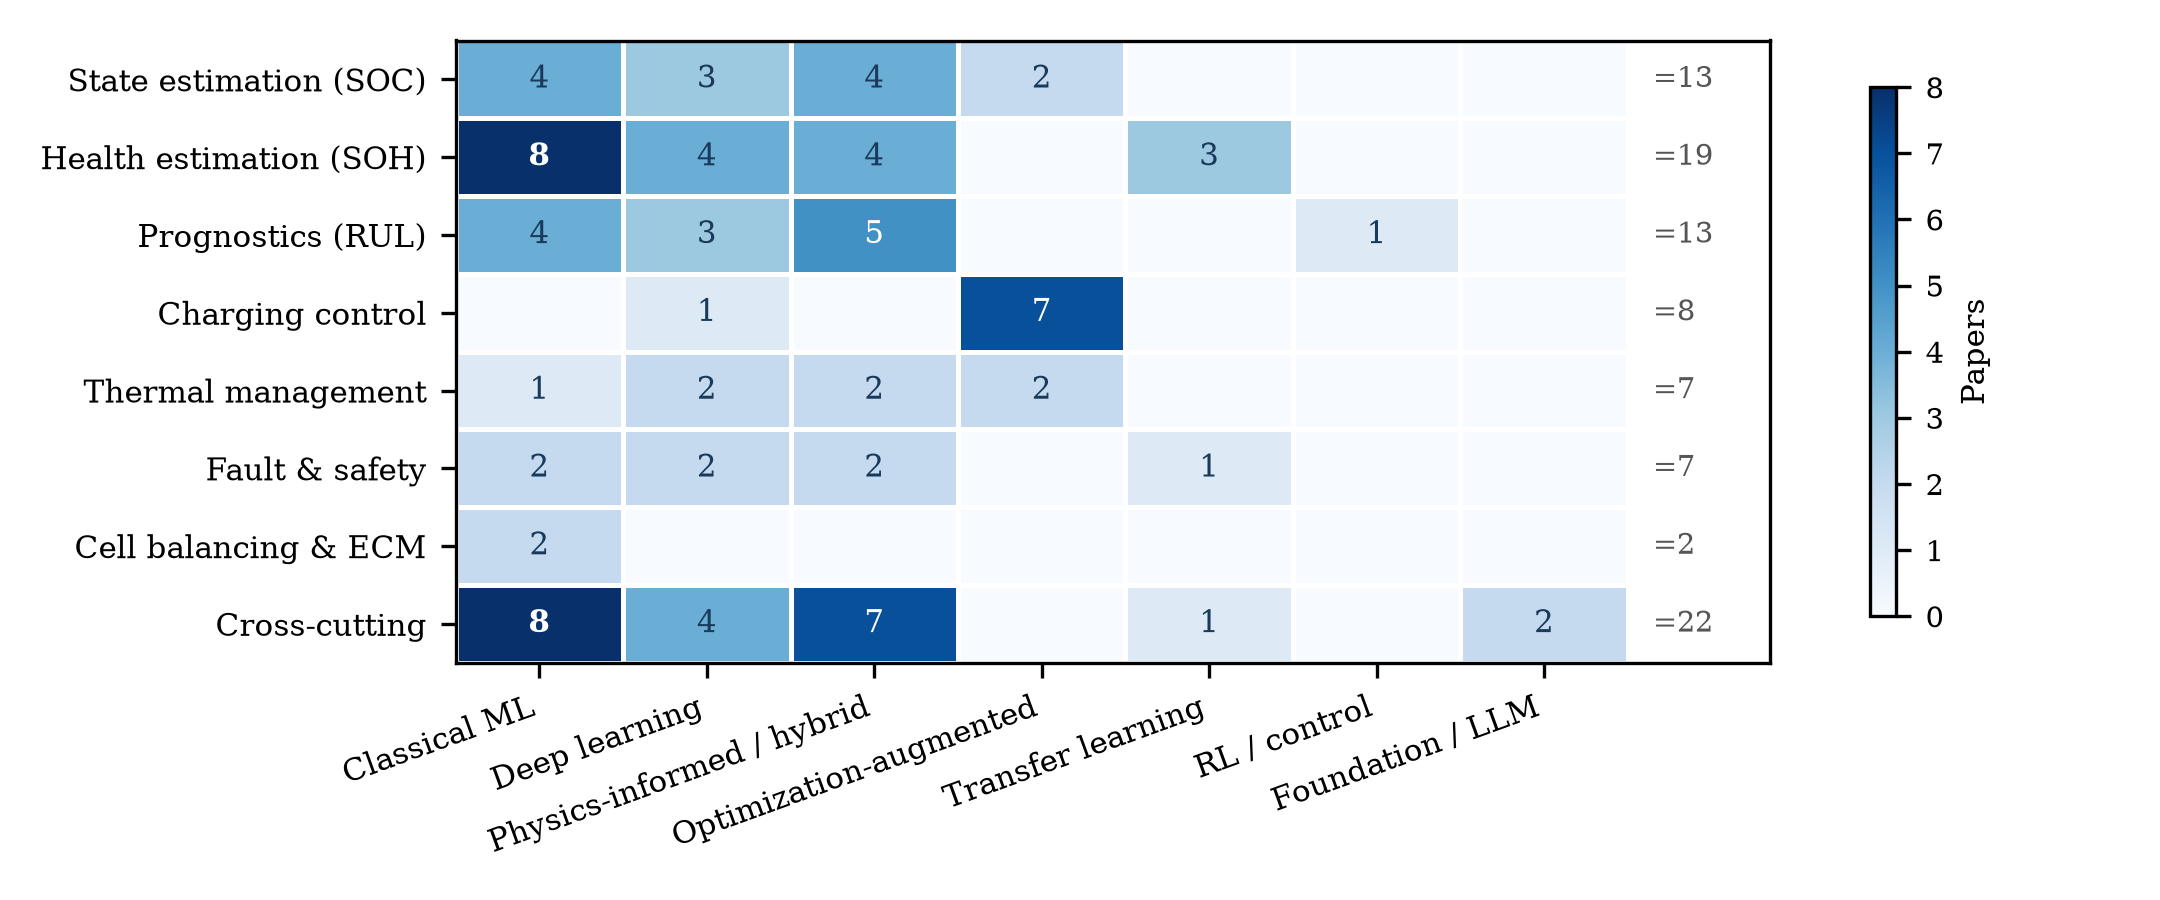
\includegraphics[width=5.3in]{figs/fig1_function_method_map.png}
\caption{The corpus mapped across battery-management functions and method families (91 primary-application papers; the 12 corpus reviews are excluded). The ``of which reviews'' column of Table II states the reconciliation directly; no excluded review belongs to the physics-informed family, so that column's corpus total of 24 (Table I) is unchanged.}
\label{fig:fig1_function_method_map.png}
\end{figure*}

\section{Review Methodology}

\subsection{Search strategy}

All candidate records were retrieved programmatically from the Crossref REST API between 4 and 5 September 2026 using 30 bibliographic query strings spanning the application areas above. Queries were issued in four passes (top-cited 2020--2026; recency from mid-2024; dedicated 2020--2022 and 2023 windows), yielding 3,000 records; after DOI-based deduplication (1,450 duplicates removed), 1,550 unique records remained. Six landmark studies --- including \cite{r3} and \cite{r2} --- were additionally safeguarded as forced seeds: five were retrieved and verified individually because citation-sorted retrieval had crowded them out, and one was already among the top-cited hits. Two properties should be stated plainly. The Crossref registry is a metadata registry, not a discovery engine like Scopus or Web of Science; it was chosen so that every included record is individually verifiable by direct DOI resolution, at the cost of a recall floor. Citation ordering also favors established English-language work; all trend statements therefore describe this citation-weighted, journal-article sample rather than the field in the aggregate.

\subsection{Screening and selection}

The screening funnel is shown in Fig. 2. A title-level relevance gate requiring both battery-related and machine-learning terminology retained 883 records and excluded 667 (predominantly adjacent-field papers that surfaced through loose matching). Venue and document-type screening removed 84 records --- conference abstracts and proceedings series, preprint servers, and non-scholarly venues --- leaving 799 eligible records. A function-quota selection step drew 107 candidate articles balanced across the eight management functions and publication years, with the six landmark seeds included in that count (one already captured by the searches, five retrieved and verified individually). Full-text curation excluded 19 records (corrigenda, misindexed records, scope mismatches, and quota-driven trimming of over-represented clusters) while 15 targeted additions were made from the screened pool for under-represented themes --- a net $-$4 that yields the final corpus of 103 studies. Inclusion required a peer-reviewed journal article on a battery subject with machine learning as a substantive component (2020--2026, plus one 2019 field-defining seed), verified by direct Crossref DOI resolution; review-only papers were admitted only into the cross-cutting cluster, capped at 12 studies.

\begin{figure*}[!t]
\centering
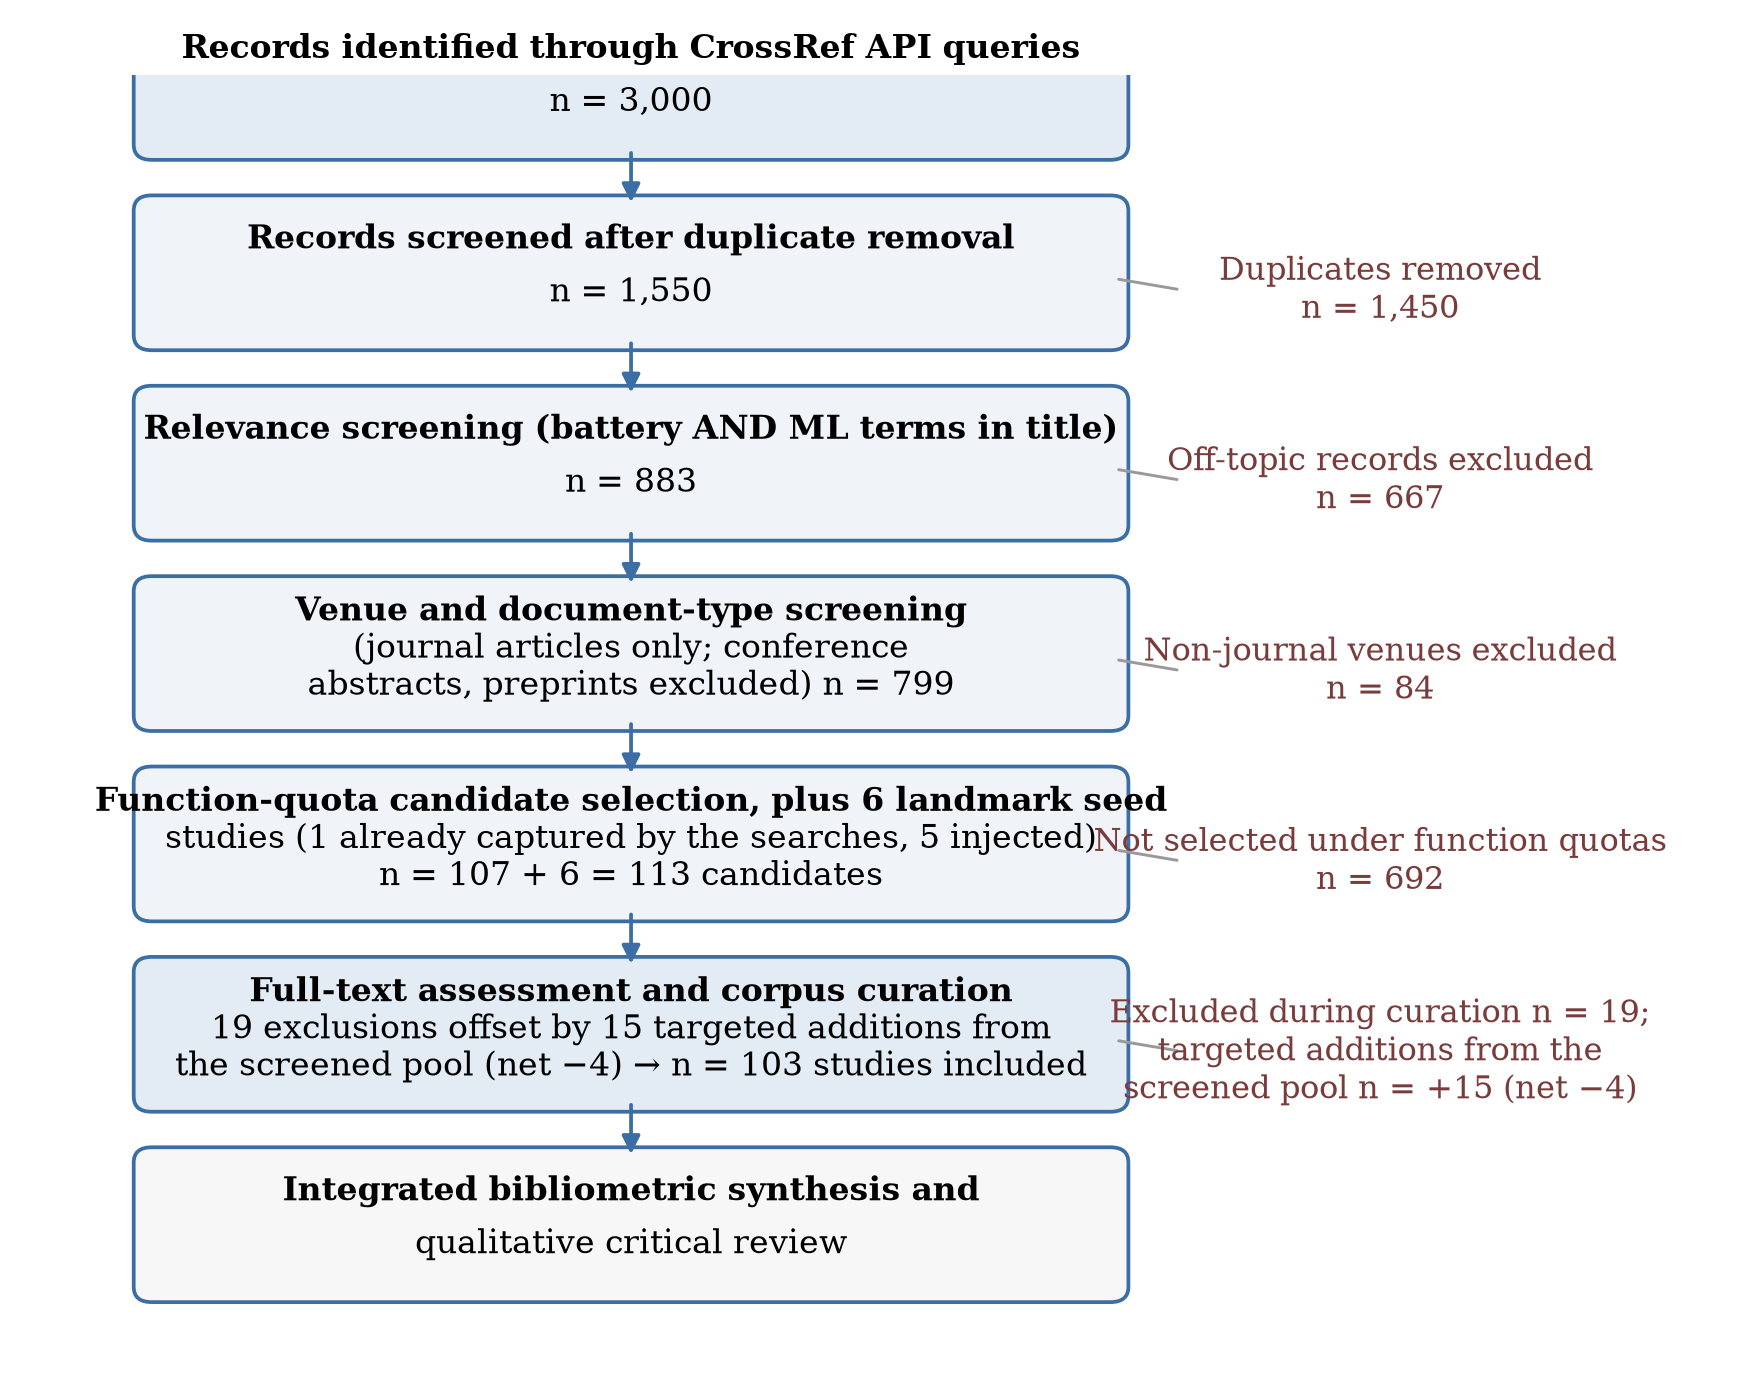
\includegraphics[width=4.9in]{figs/fig2_prisma.png}
\caption{Study-selection flowchart. Records were retrieved from the Crossref REST API on 4--5 September 2026, deduplicated, screened at title level for battery and machine-learning relevance, screened at venue and document-type level, and curated to the final 103-study corpus.}
\label{fig:fig2_prisma.png}
\end{figure*}

\subsection{Classification framework and limitations}

Each paper was classified along six fields: management function (eight values, including a cross-cutting cluster); dominant method family (classical ML, deep learning, physics-informed/hybrid, optimization-augmented, reinforcement/control learning, transfer learning, foundation models/LLMs, review); chemistry; primary data source; validation approach; and a coded summary of the headline finding and principal limitation. Three terms are used consistently: a \textit{corpus paper} is any of the 103 included studies; a \textit{primary study} (or \textit{primary-application paper}) is one of the 91 whose contribution is a primary application rather than a review. Classification was performed by the lead author with conservative coding; a co-author verification pass reviewed all 103 classifications, but because it was corrective rather than an independent blind double-coding, we claim no inter-rater agreement statistic --- the counts in Section III should be read as one documented coding of the corpus, and the complete dataset is released so that independent coders can check or extend it. The synthesis proceeds on two tracks: quantitative cross-tabulations generated programmatically from the released dataset (Section III), and qualitative function-by-function critique (Sections IV--VIII). The methodology's limitations are acknowledged: Crossref coverage excludes influential conference papers; title-level screening can miss relevant work; citation ranking privileges high-profile venues; and no formal reliability statistic is available. These are the reasons this paper describes itself as a scoping review with bibliometric classification rather than a meta-analysis.

\section{Corpus Overview and Five-Year Evolution}

\subsection{Publication trend and method-family evolution}

The corpus spans 2019--2026 (9, 13, 13, 22, 20, 18, and 7 papers per year from 2020 onward, plus the 2019 seed; Fig. 3), subject to the caveats that it is a curated sample favoring highly cited and recent work and that citation counts over-weight older publications. The defining meta-finding is the compositional shift in method families (Fig. 3, Table I). Classical ML --- Gaussian process regression, support vector machines, ensembles, and shallow networks on engineered features --- contributes 11 of the 23 papers published from 2019 through 2021. Deep sequence models rise through 2022--2023 and remain the largest family for prediction tasks. Physics-informed and hybrid model--data learning becomes the modal family by 2024--2026: counted year by year, it contributes 1, 2, 3, 4, 5, 4, and 5 papers --- 14 of its 24 corpus papers fall in 2024--2026, and it is the largest component of the 7 papers published in 2026 (Table II gives corpus-wide totals). Optimization-augmented learning (Bayesian optimization, surrogate-assisted and meta-heuristic schemes) peaks in 2023--2024 (11 papers); transfer learning accelerates in 2024--2025 (5 papers); reinforcement learning remains scarce but visible (1 corpus paper); and the first foundation-model and LLM-based studies appear in 2025--2026 (2 papers) \cite{r14}\cite{r15}. Two qualifications matter: the families are not mutually exclusive (a PSO-tuned LSTM is both deep learning and optimization-augmented), so the composition understates method mixing; and physics-informed papers are, on average, validated no more stringently than others --- if anything somewhat less stringently, a point quantified in Section III-D.

\begin{figure*}[!t]
\centering
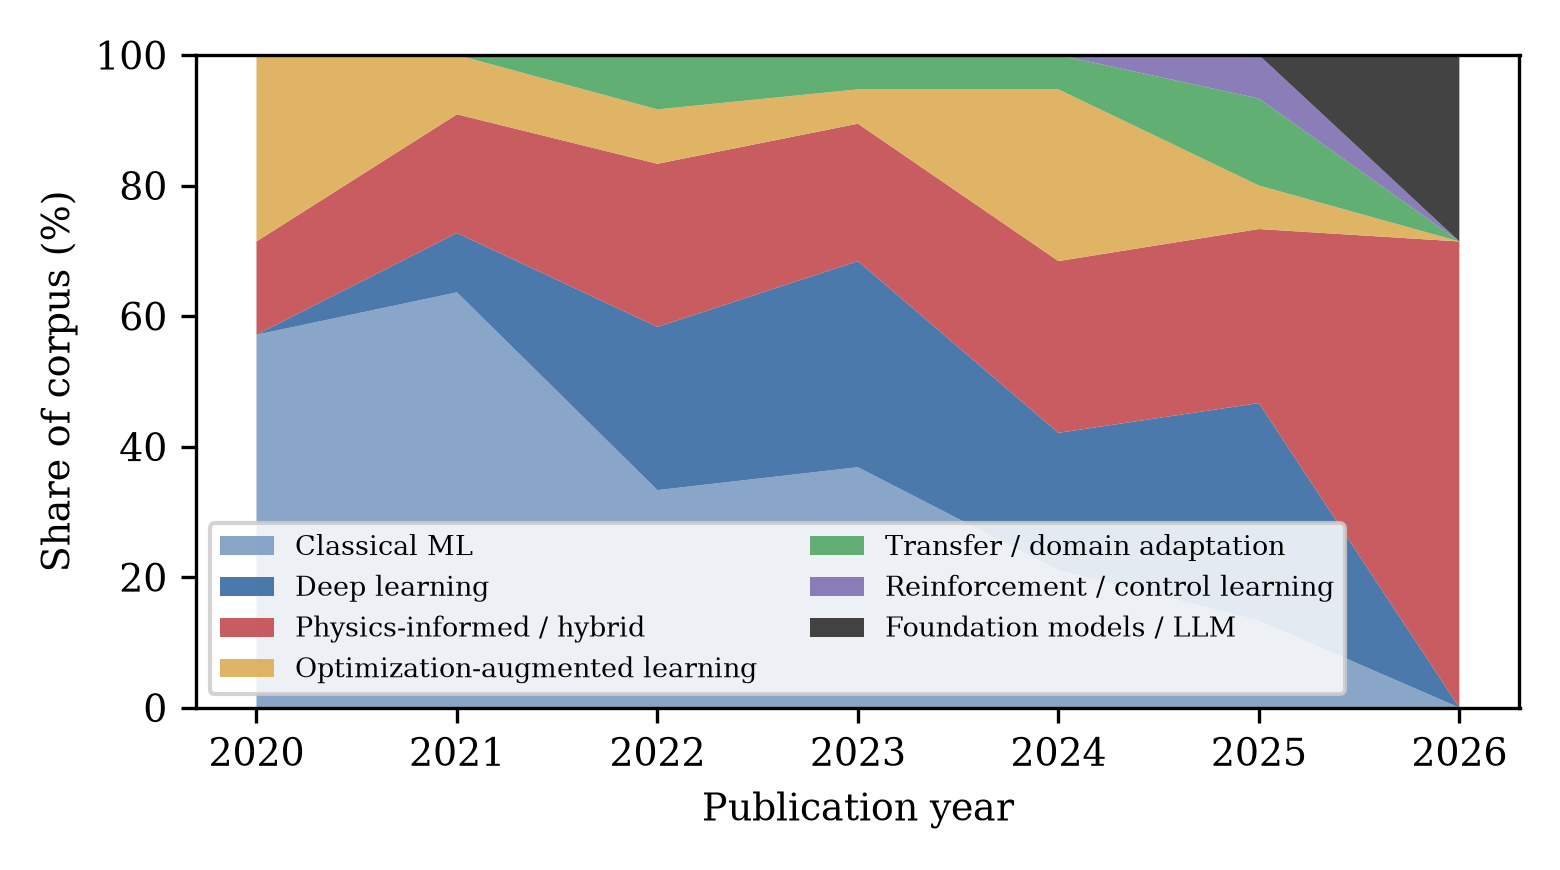
\includegraphics[width=4.4in]{figs/fig3_method_evolution.png}
\caption{Evolution of method-family shares in the corpus by publication year. The 2019 seed (classical ML) is omitted for scale.}
\label{fig:fig3_method_evolution.png}
\end{figure*}

\begin{table*}[!t]
\caption{Method families in the corpus: representative techniques, strengths, and limitations}
\label{tab:TABLE_METH}
\centering
\footnotesize
\begin{tabular}{|p{0.81in}|p{0.37in}|p{2.03in}|p{1.62in}|p{1.57in}|}
\hline
\textbf{Method family} & \textbf{Papers} & \textbf{Representative techniques} & \textbf{Strengths} & \textbf{Limitations} \\
\hline
Classical ML & 29 & Gaussian process regression, SVM/SVR, ensembles, shallow networks on engineered features & Calibrated uncertainty; small-data friendly; cheap to embed & Feature engineering is manual; ceilings under complex dynamics \\
Deep learning & 19 & LSTM/GRU, CNN, attention/Transformer, autoencoders, graph networks & Learns features from raw curves; strong trajectory modeling & Data-hungry; weak extrapolation; opaque \\
Physics-informed / hybrid & 24 & PINNs, physics-constrained autoencoders, filter-embedded networks, multiphysics fusion & Structure aids extrapolation; reduced data demand & Inherits simplified-model bias; harder to train \\
Optimization-augmented & 11 & Bayesian optimization, surrogate-assisted multi-objective design, meta-heuristic-tuned networks & Sample-efficient protocol discovery; explicit trade-off handling & Offline tuning cost; surrogate bias \\
Transfer / domain adaptation & 5 & Domain-adversarial training, fine-tuning across chemistry/protocol & Directly targets the generalization gap & Negative transfer; needs shared protocols \\
Reinforcement / control learning & 1 & Deep-RL prognostic model selection & Adaptive decision-making along trajectories & Training stability; scarce hardware validation \\
Foundation models / LLM & 2 & Domain-tuned LLM agents for risk analysis and orchestration & Reasoning over heterogeneous text/system context & Hallucination risk; latency and cost \\
Review / perspective & 12 & Narrative and systematic syntheses & Maps the field; identifies shared gaps & No primary validation \\
\hline
\end{tabular}
\end{table*}

\subsection{Application-area distribution}

Functionally, the corpus is dominated by the health-prognostics complex: health estimation (20 papers) and remaining-useful-life prognostics (15) together account for 34\% of the 103-paper corpus, followed by the cross-cutting cluster (24), state estimation (17), fault and safety (9), charging control (8), thermal management (8), and cell balancing (2) (Fig. 1; Table III gives the composition by year, with the review reconciliation; Table IV maps representative studies across all functions). This concentration mirrors publication-volume patterns in the wider literature and the commercial pull of lifetime prediction for warranties and second-life markets. The thin representation of cell balancing is telling: balancing remains dominated by classical control practice, and the corpus's most-cited balancing-related result is the demonstration that routine balancing can be dispensed with in well-managed packs, reducing hazardous lithium-plating side reactions \cite{r27}. Venue concentration is equally marked --- the Journal of Energy Storage (14 papers), Energy (13), and Applied Energy (9) head the corpus --- a sign that impact is currently demonstrated in application terms rather than in methodological novelty.

\begin{table*}[!t]
\caption{Corpus composition: management function by publication year. The Reviews column counts the 12 method-family reviews; Primary = Total $-$ Reviews gives the primary-application counts used in Fig. 1.}
\label{tab:TABLE2}
\centering
\footnotesize
\begin{tabular}{|p{1.64in}|p{0.32in}|p{0.32in}|p{0.32in}|p{0.32in}|p{0.32in}|p{0.32in}|p{0.32in}|p{0.32in}|p{0.36in}|p{0.50in}|p{0.50in}|}
\hline
\textbf{Function} & \textbf{'19} & \textbf{'20} & \textbf{'21} & \textbf{'22} & \textbf{'23} & \textbf{'24} & \textbf{'25} & \textbf{'26} & \textbf{Total} & \textbf{Reviews} & \textbf{Primary} \\
\hline
Cell balancing \& ECM & 0 & 0 & 0 & 0 & 1 & 1 & 0 & 0 & 2 & 0 & 2 \\
Charging control & 0 & 2 & 0 & 0 & 2 & 3 & 1 & 0 & 8 & 0 & 8 \\
Cross-cutting & 0 & 1 & 0 & 6 & 8 & 3 & 2 & 4 & 24 & 2 & 22 \\
Fault \& safety & 0 & 0 & 2 & 0 & 2 & 3 & 2 & 0 & 9 & 2 & 7 \\
Health estimation (SOH) & 0 & 2 & 3 & 2 & 4 & 3 & 4 & 2 & 20 & 1 & 19 \\
Prognostics (RUL) & 1 & 1 & 3 & 2 & 1 & 1 & 6 & 0 & 15 & 2 & 13 \\
State estimation (SOC) & 0 & 3 & 4 & 2 & 1 & 5 & 2 & 0 & 17 & 4 & 13 \\
Thermal management & 0 & 0 & 1 & 1 & 3 & 1 & 1 & 1 & 8 & 1 & 7 \\
Total & 1 & 9 & 13 & 13 & 22 & 20 & 18 & 7 & 103 & 12 & 91 \\
\hline
\hline
\end{tabular}
\end{table*}

\subsection{Data landscape and validation practice}

The data underpinning the corpus are strikingly concentrated: 36 papers rest on laboratory cycling of the authors' own cells; the public Severson/Toyota--MIT--Stanford (MATR) dataset alone supports 11, NASA and CALCE 6 each, and laboratory impedance spectroscopy 6; 10 papers use real vehicle or fleet data as their primary source --- a distinct measure from the 9 studies validated online or on fleets, with eight overlapping; 12 are simulation-based; and 15 are reviews or perspectives. Chemistry reporting is similarly skewed: 53 papers work on NMC-based cells and 15 on LFP, leaving sodium-ion, solid-state, and high-temperature systems nearly absent from the ML-management literature. Validation practice is arguably the field's most consequential weakness. Cross-cell holdout --- the strongest common laboratory protocol --- accounts for 24 papers, and cross-chemistry or cross-domain transfer studies for 10; but within-cell splits (12 papers) and unsupervised k-fold cross-validation (5) leak trajectory information between train and test, producing optimistic errors that do not survive cell-to-cell variability. Only 9 studies validate a system online or on fleet data, and only 7 validate across chemistries. Crossing validation practice with method family substantiates the remark in Section III-A with numbers: 13 of the 24 physics-informed/hybrid papers (54\%) use one of the strong protocols, against 49 of the other 67 primary-application papers (73\%) --- a physics prior does not, in itself, buy validation rigor.

The benchmark concentration can be stated as a metric (Fig. 4). Across 2019--2026, 23 corpus papers --- more than a fifth of the primary-application corpus --- rest on the same three public benchmarks. Because these benchmarks together contain on the order of a few hundred cells, the field's effective empirical sample has grown far more slowly than its publication count: output rose from single digits per year in 2019--2020 to 18--22 papers per year in 2023--2024, while benchmark reuse kept pace step for step. We call this pattern benchmark saturation: the empirical base on which the community calibrates and compares estimators is approximately fixed while the literature multiplies on top of it, inflating apparent comparability and hiding dataset-specific failure modes.

\begin{figure*}[!t]
\centering
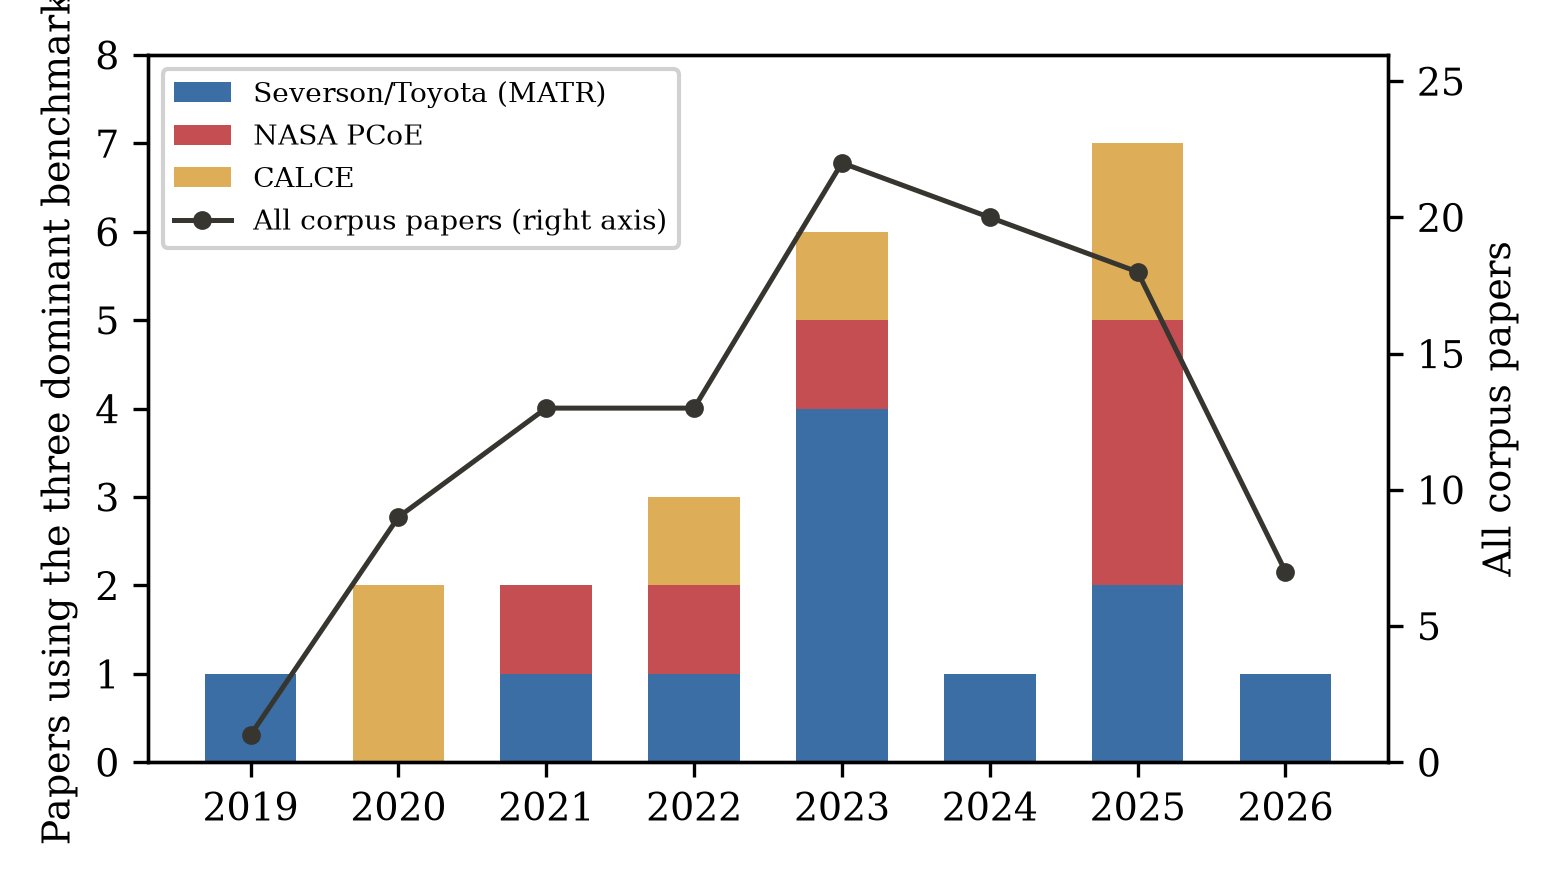
\includegraphics[width=4.2in]{figs/fig7_dataset_saturation.png}
\caption{Benchmark saturation. Papers using the three dominant public benchmarks per year (stacked bars, left axis) against total corpus output per year (line, right axis).}
\label{fig:fig7_dataset_saturation.png}
\end{figure*}

\subsection{Sensitivity analysis: does the journal-only corpus understate validation practice?}

Because the corpus excludes conference proceedings --- a major venue for control-oriented BMS work (ACC, ECC, CCDC, APEC, VPPC, ITEC) --- the validation findings could in principle be a venue-selection artifact. To test this, we curated a sensitivity set of 14 machine-learning battery papers from six control and transportation-electrification venues (2019--2025), retrieved by venue-scoped Crossref queries, restricted to proceedings articles, ranked by citation count, and verified by the same DOI-resolution procedure as the main corpus (released as conference\_sensitivity.csv). Validation practice was classified conservatively from the indexed abstracts (Table III). The result supports representativeness rather than a venue gap: only 2 of the 14 conference papers (14\%) state hardware or experimental validation in their indexed abstracts, 2 rest on public datasets, and 4 describe simulation-level validation --- against 19 of the 91 primary-application journal papers (21\%) with experimental-hardware demonstrations and a 68\% strong-protocol share. Abstract-level transparency about validation is, if anything, lower on the conference path. Two caveats bound this finding: conference abstracts are frequently truncated in bibliographic indexes, so the comparison measures stated evidence rather than underlying practice; and the set is a curated sample, not a census. Within those bounds, the journal-only corpus does not understate the field's validation transparency --- and neither venue type reports validation systematically, which strengthens the case for the reporting standards proposed in Section IX.

\begin{table*}[!t]
\caption{Conference sensitivity set: 14 machine-learning battery papers from control and transportation-electrification venues (2019--2025), Crossref-verified, with validation evidence stated in their indexed abstracts.}
\label{tab:TABLE_CONF}
\centering
\footnotesize
\begin{tabular}{|p{0.53in}|p{0.48in}|p{3.50in}|p{2.01in}|}
\hline
\textbf{Venue (year)} & \textbf{Function} & \textbf{Method family (short)} & \textbf{Validation evidence stated in indexed abstract} \\
\hline
ITEC 2019 & SOC & LSTM recurrent network \cite{r28} & Not stated \\
VPPC 2021 & SOH & ML ensemble \cite{r29} & Public dataset \\
ITEC 2022 & SOC+SOH & Dual extended Kalman filter \cite{r30} & Not stated \\
ACC 2023 & SOC+SOH & Real-time estimator + batch least squares \cite{r31} & Not stated \\
ACC 2021 & SOC & Multiple-model adaptive estimation \cite{r32} & Simulation-level \\
ITEC 2023 & SOH & Histogram data + PCA + regression \cite{r33} & Public dataset \\
APEC 2023 & Overview & Review of ML-enabled estimation \cite{r34} & Not applicable \\
ECC 2021 & SOH & Reinforcement learning + observer \cite{r35} & Not stated \\
CCDC 2022 & SOH & CNN-BiLSTM transfer learning \cite{r36} & Hardware (stated); public data \\
VPPC 2019 & SOC & SVR + PCA with dual-polarization model \cite{r37} & Not stated \\
ACC 2024 & SOC+SOH & EKF critique and improvement \cite{r38} & Simulation-level \\
VPPC 2022 & Prognostics & ML on aging data \cite{r39} & Hardware (stated) \\
VPPC 2019 & SOC & Kalman filter on reduced electrochemical model \cite{r40} & Simulation-level \\
VPPC 2021 & SOC & Computationally efficient neural network \cite{r41} & Simulation-level \\
\hline
\end{tabular}
\end{table*}

\section{Machine Learning for Battery State Estimation}

SOC estimation is the most mature BMS function, and the corpus shows how machine learning entered it. The early pattern pairs learning with classical estimation: Gaussian process regression for pack-level SOC with native uncertainty quantification \cite{r42}, and --- most influentially --- recurrent networks embedded in unscented Kalman filters, where the LSTM supplies a learned observation model and the filter recursive correction \cite{r5}. A second generation tuned network structure itself: particle-swarm-optimized LSTM improved accuracy and noise robustness \cite{r43}, and evolutionary-assisted CNN--BiLSTM hybrids report sub-1\% drive-cycle errors \cite{r44}. Simulation-informed training pipelines substitute automotive-accurate simulated data for exhaustive cell testing \cite{r45}, comparative benchmarks on standard drive cycles weigh ML regression families \cite{r46}, pack heterogeneity is addressed by joint pack-SOC and cell-inconsistency estimation with balancing-aware formulations \cite{r47}, and unified frameworks estimate SOH and SOC jointly from partial charging data \cite{r48}, and large-format applications extend estimation to containerized storage strings \cite{r49}, with comparative benchmarks weighing accuracy against embedded compute budgets \cite{r50}\cite{r51}.

The most substantive recent shift is toward hybrid schemes in which a filter, an equivalent-circuit model, or a physics prior constrains the learner: GA-optimized LSTM coupled with improved adaptive Kalman filtering reaches low error under measurement noise that breaks pure-network estimators \cite{r52}; equivalent-circuit-informed ML on impedance features estimates SOC across temperatures \cite{r53}; and physics-informed recurrent structures embed battery dynamics directly into the training objective \cite{r10}. These schemes trade engineering complexity for extrapolation behavior --- the property that matters most onboard. Yet 13 of the 17 corpus SOC papers rest on laboratory-scale data and 12 on a single chemistry, and only one demonstrates fleet-scale operation \cite{r49}; benchmark heterogeneity makes cross-paper comparison nearly meaningless \cite{r20}\cite{r17}. The laboratory problem is largely solved; the deployment problem --- guaranteed accuracy on arbitrary packs over full aging --- is not.

\section{Machine Learning for Health Estimation and Prognostics}

SOH estimation and RUL prediction form the largest functional block of the corpus (35 papers). The founding pattern is classical: extract health-sensitive features from partial charge or discharge curves, then regress with Gaussian process or similar shallow models --- incremental-capacity analysis with explicit uncertainty bounds \cite{r54}, differential thermal voltammetry \cite{r55}, and Gaussian-process classification of impedance spectra that identifies degradation modes \cite{r56}, and deep Gaussian processes coupling prognosis with degradation-mode identification \cite{r57}. Measurement relaxations followed: random partial charging data proved sufficient for accurate SOH \cite{r58}, and charging-segment adjustment refined features for vehicle-level use \cite{r59}. The landmark systematization is Roman et al.'s 179-cell pipeline showing that relaxed charge-curve features support accurate SOH estimation across a heterogeneous commercial fleet \cite{r60}.

Deep architectures entered as sequence models over capacity-fade trajectories and representation learners over raw curves: graph convolutional networks fusing multiple health indicators \cite{r7}, graph networks over partial discharge curves \cite{r61}, BiLSTM--Transformer hybrids under fast-charging stress \cite{r8}, hybrid-fusion networks for real-time prediction streams \cite{r62}, and interpretable deep learning with transparency mechanisms \cite{r63}. Field-data studies absorb real-vehicle noise \cite{r6} and estimate pack-level SOH from fleet streams \cite{r64}, while deep models estimate SOH without additional degradation experiments by learning trajectory features that generalize across chemistries \cite{r65}. Early-life prediction --- forecasting lifetime from the first cycles --- compresses test times from months to days \cite{r3}\cite{r66}\cite{r67}, hybrid physics-plus-learned models give early RUL from limited cycles \cite{r68}, extends to lithium-metal chemistries \cite{r69}, and now runs on embedded boards in real time \cite{r70}.

The prognostics cluster shows the clearest physics-informed turn: physics-informed online degradation models \cite{r71}, hybrid reinforcement learning that reduces the data demand of SOH estimation \cite{r72}, a generalizable PINN from limited early-cycle data \cite{r73}, EIS-informed physics-constrained networks \cite{r74}, a generic physics-informed RUL framework for small early-life samples \cite{r75}, multi-feature hybrids across datasets \cite{r76}, recurrent networks anticipating uncertain duty \cite{r77}, and signal-decomposition hybrids on noisy capacity series \cite{r78}. Transfer learning attacks generalization directly: domain-adversarial training across operating conditions \cite{r11}, deep transfer with partial charging curves across cell types \cite{r12}, transfer under fast-charging protocols \cite{r79}, cross-chemistry EIS estimation \cite{r80}, and a general framework quantifying the laboratory-to-fleet domain gap \cite{r81}. The critical assessment: accuracy claims cluster around 1--2\% SOH error, but they are established overwhelmingly on public benchmark cells --- 10 of the 35 studies in this complex use within-cell or k-fold validation (17 corpus-wide) --- and the transfer-learning papers, the honest exception, reveal how much shift remains unaddressed. SOH estimation under controlled conditions is approaching incremental returns; calibrated lifetime and safety margins for arbitrary packs in the field remain open \cite{r2}\cite{r19}.

\begin{table*}[!t]
\caption{Representative corpus studies by management function and method family. Entries gloss each study as: study summary (data basis; headline contribution). References in brackets refer to the numbered list.}
\label{tab:TABLE_REP}
\centering
\footnotesize
\begin{tabular}{|p{1.01in}|p{2.11in}|p{3.52in}|}
\hline
\textbf{Function} & \textbf{Method family} & \textbf{Representative studies (data; contribution)} \\
\hline
State estimation (SOC) & Filter-embedded learning; meta-heuristic DL & LSTM+UKF embedded estimator (laboratory cells; learned observation model in a UKF) \cite{r5}; PSO-LSTM (laboratory cells; meta-heuristically tuned recurrent SOC) \cite{r43}; GA-LSTM with adaptive Kalman filtering (laboratory cells; low error under noise) \cite{r52} \\
Health estimation (SOH) & Classical ML; deep learning; transfer learning & ML pipeline over 179 cells (own cell fleet; relaxed charge-curve features) \cite{r60}; deep learning without extra degradation experiments (public MATR dataset; cross-chemistry generalization) \cite{r65}; real-world vehicle SOH (fleet data; field-noise robustness) \cite{r6} \\
Prognostics (RUL) & Classical ML; physics-informed; RL & Early-life cycle prediction (public MATR dataset; about 9\% median test error) \cite{r3}; physics-informed early-cycle RUL (multiple datasets; small-data prognosis) \cite{r75}; deep-RL prognostic model fusion (public NASA dataset; adaptive model selection) \cite{r13} \\
Charging control & Bayesian optimization; mechanism-aware control & Closed-loop Bayesian protocol optimization (hardware prototype; 2.5 versus 18 months to a protocol) \cite{r4}; plating-perceiving fast charging (hardware prototype; plating-free protocols) \cite{r82}; ensemble-surrogate charging optimization (laboratory cells; multi-objective strategies) \cite{r83} \\
Thermal management & ANN surrogate; physics-informed; optimization & ANN temperature prediction (laboratory cells; low-error thermal model) \cite{r84}; PINN heat-generation estimation (simulation; embedded thermal physics) \cite{r9}; ML-assisted BTMS design (simulation; multi-objective cooling design) \cite{r85} \\
Fault \& safety & Shallow ML; multiphysics + ML; transfer learning & SVM fault diagnosis (hardware prototype; sensor and connection faults) \cite{r86}; multiphysics-ML runaway prediction (simulation and hardware; module-level hazard) \cite{r87}; cross-fleet runaway-diagnosis transfer (fleet data; small-sample diagnosis) \cite{r88} \\
Cross-cutting & Physics-informed; XAI; digital twin; LLM & EIS diagnostics PINN review (multiple studies; paradigm synthesis) \cite{r21}; uncertainty-aware early-life prediction (public MATR dataset; calibrated forecasts) \cite{r89}; LLM vehicle-cloud management (fleet data; orchestration layer) \cite{r15} \\
\hline
\end{tabular}
\end{table*}

\section{Machine Learning for Charging Control and Optimization}

Charging control is the function where machine learning has changed experimental practice most directly. The defining result is Attia et al.: a Bayesian optimization loop identified fast-charging protocols within 2.5 months, against roughly 18 months of manual search \cite{r4}. Ensemble surrogates make multi-objective strategy optimization tractable \cite{r83}, and Bayesian fast-charging optimization reduces charge time under degradation constraints \cite{r90}. A second line embeds degradation mechanisms into the decision itself: machine-learning fast charging that perceives and regulates internal lithium-plating onset enables plating-free rapid protocols \cite{r82}, adaptive multistage schemes adjust stage boundaries against measured degradation \cite{r91}, module-level optimization manages temperature gradients \cite{r92}, and pack-level extensions coordinate balance-aware charging \cite{r93}\cite{r94}.

The deployment gap is most concrete here: of the eight charging papers, one is a large-scale closed-loop hardware campaign, three validate on laboratory hardware, and the rest are simulation-only. The unsolved problem is certifiable learning-based charging --- which is why mechanism-aware schemes such as plating-perception control \cite{r82} are the cluster's most deployment-relevant results.

\section{Machine Learning for Thermal Management, Faults and Safety}

Thermal management (8 papers) divides by purpose. For estimation, ANN models predict cell temperature across operating conditions \cite{r84} and internal-temperature sensing extends to ultrahigh-rate discharge where surface measurement fails \cite{r95}. For design, ML surrogates amortize expensive CFD evaluation across optimization loops \cite{r96}\cite{r85}, with experimentally validated parallel-liquid-cooling designs closing the loop \cite{r97}. For control, ANN controllers demonstrate parasitic-load reductions in simulation \cite{r98} --- but no corpus paper closes this loop on hardware, leaving thermal control where charging control was five years ago. Physics-informed heat-generation estimation embeds thermal priors into the learning problem \cite{r9}, and the cluster is consolidated by a state-of-the-art review \cite{r25}.

Fault and safety applications (9 papers) divide into diagnosis of realized faults and prediction of impending hazards: grid-search-optimized SVMs classify sensor and connection faults \cite{r86}, curvilinear-distance methods detect multiple pack fault types in operating fleets \cite{r99}, and multi-scenario deep anomaly detection covers real EV operating envelopes \cite{r100}; force-signal deep learning catches lithium-plating-type defects at manufacturing \cite{r101}. The hazard-prediction side is increasingly model-based: multiphysics models coupled with ML predict module-level thermal-runaway progression \cite{r87}, a multiphysics-informed DeepONet augments scarce experimental events with virtual data \cite{r102}, and multi-source domain transfer moves thermal-runaway diagnosis across fleets with small target samples \cite{r88}. The reviews in this cluster are candid that laboratory fault diagnosis has historically failed to transfer to real vehicles \cite{r24}\cite{r23}; the fleet-data anomaly-detection studies are therefore the cluster's most valuable trend, even though label scarcity for rare faults keeps evaluation largely qualitative.

\section{Cross-Cutting Directions}

\subsection{Physics-informed learning, interpretability, and uncertainty}

Physics-informed and hybrid model--data learning is the corpus's largest methodological theme (24 papers across all functions) --- in state estimation \cite{r10}\cite{r103}, heat-generation estimation \cite{r9}, prognostics \cite{r71}, and impedance-based diagnostics \cite{r21}, with physics-constrained autoencoders improving health prediction over purely learned counterparts \cite{r104} and a physical-plus-data-driven fusion literature for internal-state estimation \cite{r105}. The caution is that most physics-informed studies embed simplified physics --- equivalent-circuit or reduced electrochemical models --- so the hybrid inherits model bias even as it gains structure, and its validation is no stronger than that of purely data-driven peers (Section III-D). A smaller but consequential cluster makes learning systems inspectable: explainability-driven feature selection improves estimator robustness \cite{r106}, interpretable ML links manufacturing coating parameters to cell capacity \cite{r107}, interpretable hybrid ML untangles degradation chemistries in lithium--sulfur cells \cite{r108}, and uncertainty-aware models deliver calibrated early-life predictions \cite{r89}. For safety cases only calibrated uncertainty has a route into certification; attribution supports debugging.

\subsection{Digital twins, cloud BMS, and new sensing}

System-level architecture is emerging as a research object: digital twins track individual battery aging through incremental learning \cite{r109} and couple LSTM surrogates with real-time thermal observation \cite{r110}; cloud platforms perform in-situ life prediction at fleet scale \cite{r111}; second-life workflows use impedance-based accelerated SOH estimation to triage retired packs \cite{r112}, and learned battery models with numerical search estimate real-time state-of-power \cite{r113}. Non-electrical sensing broadens the measurement base --- ultrasonic signatures provide a SOC channel orthogonal to voltage sensing \cite{r114} --- and ML mappings from equivalent-circuit parameters to electrochemical properties give classical BMS models a physically interpretable learned layer \cite{r115}. These settings differ in latency budgets, error tolerance, and update cadence, and the field is beginning to design for those differences. Production-side mapping \cite{r116}, coating interpretability \cite{r107}, and defect detection \cite{r101} complete the picture: cell quality is itself a BMS input.

\subsection{Foundation models and LLM-based management}

The corpus's youngest theme is generative: domain-specific LLMs perform risk analysis of battery energy-storage incidents \cite{r14}, and knowledge-enhanced LLM agents orchestrate vehicle-cloud battery management \cite{r15}. Because BMS software is safety-critical, this review positions foundation models not as better estimators but as orchestration layers, and Table V makes the division of labor explicit: the right-hand guardrails are normative guidance proposed here, not claims about the published studies. Two entries deserve emphasis. Failure mode: an estimator's error is a bounded number, while an LLM's failure is open-ended hallucinated text --- so LLM outputs must be restricted to structured, checkable forms and never feed protection logic as free text. Safety authority: LLM components must never hold direct cell-level protection authority; that role belongs to physics-based envelopes and calibrated estimators whose uncertainty is quantified.

\begin{table*}[!t]
\caption{Safety and verification taxonomy for foundation-model components in the BMS stack. The right-hand column is normative guidance proposed by this review, not claims about the published studies.}
\label{tab:TABLE_LLM}
\centering
\footnotesize
\begin{tabular}{|p{0.57in}|p{1.64in}|p{2.16in}|p{2.16in}|}
\hline
\textbf{Dimension} & \textbf{Classical / deep ML estimators (established practice)} & \textbf{Published LLM studies (2025--2026)} & \textbf{Required guardrail (this review)} \\
\hline
Role in the stack & Calibrated numeric estimation and detection & Incident risk analysis \cite{r14}; vehicle-cloud orchestration \cite{r15} & Estimation stays with calibrated ML; LLM coordinates, summarizes, explains \\
Grounding & Trained on domain cycling data & Domain-tuned corpora and knowledge-enhanced prompting & Retrieval over verified corpora with source citations; no ungrounded recall \\
Dominant failure mode & Bounded numeric error under distribution shift & Open-ended hallucinated text & Outputs restricted to structured, checkable forms; never free text into protection logic \\
Uncertainty & Gaussian-process / conformal intervals in a subset of studies & Not quantified in published studies & Calibrated intervals mandatory before any actuation-adjacent role \\
Latency and compute & Millisecond-class, onboard & Second-class, cloud-dependent & Offline analysis and planning only unless real-time evidence is shown \\
Safety authority & Bounded by physics envelopes and thresholds & Undefined in published studies & LLM components must never hold direct cell-level protection authority \\
\hline
\end{tabular}
\end{table*}

\section{Research Gaps, Reporting Standards, and Future Directions}

Cross-referencing the bibliometric analysis of Section III with the function-level reviews yields six structural gaps. (1) Validation practice: 17 primary studies use within-cell or unsupervised k-fold validation, and only 9 of all 103 demonstrate online or fleet use; standardized cross-cell, cross-chemistry, and lab-to-fleet transfer protocols should become reporting norms, as already practiced by the transfer-learning and general-framework studies \cite{r81}\cite{r80}. (2) Data monoculture: a single public dataset underlies 11 studies, NASA and CALCE sustain much of the rest, and 36 papers use private laboratory cells; federated learning over fleets, anonymized fleet-data releases, and multi-institution cycling campaigns --- in the spirit of the 179-cell pipeline \cite{r60} --- would diversify the evidence base, and papers should at minimum disclose split definitions, seeds, and compute budgets. (3) Edge deployment: only isolated works treat onboard compute, memory, and latency as first-class constraints \cite{r70}\cite{r117}; quantization-aware training, resource-constrained architecture search, and cloud--edge hybrid designs are the natural research program. (4) Trust: uncertainty must be calibrated rather than post-hoc \cite{r89}, interpretability must bound behavior rather than merely attribute it, and hybrid physics--data architectures are the most credible certification path because part of their behavior is analytically specified. (5) Foundation-model integration: the first LLM studies \cite{r14}\cite{r15} suggest a division of labor --- foundation models for reasoning and orchestration, conventional ML for calibrated estimation, physics models for safety envelopes --- that should be formalized with grounding and latency guarantees. (6) Under-served functions: balancing is nearly untouched beyond pack-level insight \cite{r27}, charging needs certifiable adaptive protocols, and thermal management remains simulation-dominated \cite{r25}; these are control problems where errors act on the battery, so closing them requires the safety-case machinery of gap 4 as much as new algorithms.

\begin{table}[!t]
\caption{Proposed BMS-ML reporting checklist (BMS-ML-RC), modeled on CONSORT/PRISMA reporting standards.}
\label{tab:TABLE_CHECKLIST}
\centering
\footnotesize
\begin{tabular}{|p{0.35in}|p{2.81in}|}
\hline
\textbf{\#} & \textbf{Reporting item --- what must be reported} \\
\hline
1 & Dataset identity --- exact name and version of every dataset (e.g., Severson-MATR, NASA, CALCE); download source \\
2 & Cell population --- number of cells, chemistry, manufacturer, format, and batch for every training and test set \\
3 & Sensor and sampling context --- measured channels, sampling rate, sensor class, temperature conditions \\
4 & Split protocol --- split type (within-cell / cross-cell / cross-chemistry / cross-domain) and isolation argument \\
5 & Out-of-distribution evaluation --- at least one protocol where test conditions differ from training \\
6 & Baselines --- at least one classical baseline alongside the proposed architecture, on identical data \\
7 & Randomness control --- seeds or repeated-run statistics for every stochastic result \\
8 & Uncertainty --- calibrated intervals or error bars for headline claims, not point estimates alone \\
9 & Compute budget --- training compute and inference latency/memory on the target platform \\
10 & Failure analysis --- at least one documented failure mode and its distribution \\
11 & Validation environment --- simulation, laboratory cycling, hardware prototype, or online/fleet \\
12 & Artifact availability --- data and code deposit (DOI-backed) or an explicit stated exemption \\
\hline
\end{tabular}
\end{table}

\subsection{A reporting checklist for machine-learning BMS studies}

The most concrete artifact this review can offer is procedural. Modeled on the CONSORT and PRISMA checklists, Table VI proposes a twelve-item BMS-ML reporting checklist (BMS-ML-RC): the minimum metadata a study should disclose for its accuracy claims to be comparable, reproducible, and poolable. Each item corresponds to a practice whose absence the corpus analysis showed to be distorting --- undisclosed splits, uncalibrated uncertainty, unnamed datasets, unquantified compute. We suggest journals adopt it as a submission checklist and that authors attach it to their released datasets.

\section{Conclusion}

This review has examined AI-powered battery management through a verified 103-study corpus extended by a 14-paper conference sensitivity analysis. Three conclusions stand out. First, the field has undergone a marked methodological evolution: classical feature-based learners gave way to deep sequence models, now being displaced at the frontier by physics-informed hybrids, optimization-augmented learning, transfer-learning regimes, and foundation-model components. Second, the center of gravity remains estimation, where learning systems have largely succeeded on laboratory terms; control functions remain demonstrably transformable but under-evidenced for deployment. Third, published accuracy progress is not matched by validation progress: online or fleet-level demonstration appears in fewer than one study in ten, benchmark monoculture distorts the state of the art, and physics-informed architecture does not substitute for validation rigor (54\% versus 73\% strong-protocol validation). The near-term agenda follows from these gaps directly: standardized cross-domain validation, diversified fleet data, edge-deployable architectures, calibrated uncertainty, and a strict division of labor between foundation models, calibrated estimators, and physics-based safety envelopes. If the last five years were about discovering what machine learning can estimate about a battery, the next five will be decided by what it can be trusted to do --- onboard, at fleet scale, across chemistries, and over full cell lifetimes.

\begin{thebibliography}{120}
\bibitem{r1}
M. F. Ng, J. Zhao, Q. Yan, G. J. Conduit, Z. W. Seh, ``Predicting the state of charge and health of batteries using data-driven machine learning,'' \emph{Nature Machine Intelligence}, vol. 2, no. 3, p. 161-170, 2020. doi: 10.1038/s42256-020-0156-7.
\bibitem{r2}
X. Hu, L. Xu, X. Lin, M. Pecht, ``Battery Lifetime Prognostics,'' \emph{Joule}, vol. 4, no. 2, p. 310-346, 2020. doi: 10.1016/j.joule.2019.11.018.
\bibitem{r3}
K. A. Severson, P. M. Attia, N. Jin, N. Perkins, B. Jiang, Z. Yang et al., ``Data-driven prediction of battery cycle life before capacity degradation,'' \emph{Nature Energy}, vol. 4, no. 5, p. 383-391, 2019. doi: 10.1038/s41560-019-0356-8.
\bibitem{r4}
P. M. Attia, A. Grover, N. Jin, K. A. Severson, T. M. Markov, Y. H. Liao et al., ``Closed-loop optimization of fast-charging protocols for batteries with machine learning,'' \emph{Nature}, vol. 578, no. 7795, p. 397-402, 2020. doi: 10.1038/s41586-020-1994-5.
\bibitem{r5}
F. Yang, S. Zhang, W. Li, Q. Miao, ``State-of-charge estimation of lithium-ion batteries using LSTM and UKF,'' \emph{Energy}, vol. 201, p. 117664, 2020. doi: 10.1016/j.energy.2020.117664.
\bibitem{r6}
J. Tian, X. Liu, S. Li, Z. Wei, X. Zhang, G. Xiao et al., ``Lithium-ion battery health estimation with real-world data for electric vehicles,'' \emph{Energy}, vol. 270, p. 126855, 2023. doi: 10.1016/j.energy.2023.126855.
\bibitem{r7}
Y. Wei, D. Wu, ``Prediction of state of health and remaining useful life of lithium-ion battery using graph convolutional network with dual attention mechanisms,'' \emph{Reliability Engineering \& System Safety}, vol. 230, p. 108947, 2023. doi: 10.1016/j.ress.2022.108947.
\bibitem{r8}
Z. Li, X. Zhang, W. Gao, ``State of health estimation of lithium-ion battery during fast charging process based on BiLSTM-Transformer,'' \emph{Energy}, vol. 311, p. 133418, 2024. doi: 10.1016/j.energy.2024.133418.
\bibitem{r9}
H. Pang, L. Wu, J. Liu, X. Liu, K. Liu, ``Physics-informed neural network approach for heat generation rate estimation of lithium-ion battery under various driving conditions,'' \emph{Journal of Energy Chemistry}, vol. 78, p. 1-12, 2023. doi: 10.1016/j.jechem.2022.11.036.
\bibitem{r10}
Y. Wang, X. Han, D. Guo, L. Lu, Y. Chen, M. Ouyang, ``Physics-Informed Recurrent Neural Network With Fractional-Order Gradients for State-of-Charge Estimation of Lithium-Ion Battery,'' \emph{IEEE Journal of Radio Frequency Identification}, vol. 6, p. 968-971, 2022. doi: 10.1109/jrfid.2022.3211841.
\bibitem{r11}
Z. Ye, J. Yu, ``State-of-Health Estimation for Lithium-Ion Batteries Using Domain Adversarial Transfer Learning,'' \emph{IEEE Transactions on Power Electronics}, vol. 37, no. 3, p. 3528-3543, 2022. doi: 10.1109/tpel.2021.3117788.
\bibitem{r12}
J. Yao, T. Han, ``Data-driven lithium-ion batteries capacity estimation based on deep transfer learning using partial segment of charging/discharging data,'' \emph{Energy}, vol. 271, p. 127033, 2023. doi: 10.1016/j.energy.2023.127033.
\bibitem{r13}
M. Du, Y. Zhang, Q. Miao, ``Remaining useful life prediction of lithium battery based on deep reinforcement learning fusion network,'' \emph{Reliability Engineering \& System Safety}, vol. 264, p. 111392, 2025. doi: 10.1016/j.ress.2025.111392.
\bibitem{r14}
J. Liang, H. Meng, Y. Mu, ``Domain-specific large language model-driven risk analysis of battery energy storage systems,'' \emph{Reliability Engineering \& System Safety}, vol. 274, p. 112416, 2026. doi: 10.1016/j.ress.2026.112416.
\bibitem{r15}
S. Cai, J. Chen, J. Hu, R. Huang, J. Liao, M. Wei et al., ``HA-LLM: A domain knowledge-enhanced large language model for vehicle-cloud collaborative battery health awareness,'' \emph{Energy Storage Materials}, vol. 86, p. 104983, 2026. doi: 10.1016/j.ensm.2026.104983.
\bibitem{r16}
Y. Liu, Y. He, H. Bian, W. Guo, X. Zhang, ``A review of lithium-ion battery state of charge estimation based on deep learning: Directions for improvement and future trends,'' \emph{Journal of Energy Storage}, vol. 52, p. 104664, 2022. doi: 10.1016/j.est.2022.104664.
\bibitem{r17}
Y. Wu, D. Bai, K. Zhang, Y. Li, F. Yang, ``Advancements in the estimation of the state of charge of lithium-ion battery: a comprehensive review of traditional and deep learning approaches,'' \emph{Journal of Materials Informatics}, vol. 5, no. 2, 2025. doi: 10.20517/jmi.2024.84.
\bibitem{r18}
X. Sui, S. He, S. B. Vilsen, J. Meng, R. Teodorescu, D. I. Stroe, ``A review of non-probabilistic machine learning-based state of health estimation techniques for Lithium-ion battery,'' \emph{Applied Energy}, vol. 300, p. 117346, 2021. doi: 10.1016/j.apenergy.2021.117346.
\bibitem{r19}
X. Li, D. Yu, V. Søren Byg, S. Daniel Ioan, ``The development of machine learning-based remaining useful life prediction for lithium-ion batteries,'' \emph{Journal of Energy Chemistry}, vol. 82, p. 103-121, 2023. doi: 10.1016/j.jechem.2023.03.026.
\bibitem{r20}
J. Yao, J. Kowal, ``Towards a smarter battery management system: A critical review on deep learning-based state of charge estimation of lithium-ion batteries,'' \emph{Energy and AI}, vol. 21, p. 100585, 2025. doi: 10.1016/j.egyai.2025.100585.
\bibitem{r21}
Y. H. Lin, S. J. Ruan, Y. X. Chen, Y. F. Li, ``Physics-informed deep learning for lithium-ion battery diagnostics using electrochemical impedance spectroscopy,'' \emph{Renewable and Sustainable Energy Reviews}, vol. 188, p. 113807, 2023. doi: 10.1016/j.rser.2023.113807.
\bibitem{r22}
T. Wang, K. Liu, H. Peng, X. Liu, ``Interpretable Machine Learning for Battery Prognosis: Retrospect and Prospect,'' \emph{Advanced Energy Materials}, vol. 15, no. 48, Art. no. e03067, 2025. doi: 10.1002/aenm.202503067.
\bibitem{r23}
A. Samanta, S. Chowdhuri, S. S. Williamson, ``Machine Learning-Based Data-Driven Fault Detection/Diagnosis of Lithium-Ion Battery: A Critical Review,'' \emph{Electronics}, vol. 10, no. 11, p. 1309, 2021. doi: 10.3390/electronics10111309.
\bibitem{r24}
Q. Yu, C. Wang, J. Li, R. Xiong, M. Pecht, ``Challenges and outlook for lithium-ion battery fault diagnosis methods from the laboratory to real world applications,'' \emph{eTransportation}, vol. 17, p. 100254, 2023. doi: 10.1016/j.etran.2023.100254.
\bibitem{r25}
A. Li, J. Weng, A. C. Y. Yuen, W. Wang, H. Liu, E. W. M. Lee et al., ``Machine learning assisted advanced battery thermal management system: A state-of-the-art review,'' \emph{Journal of Energy Storage}, vol. 60, p. 106688, 2023. doi: 10.1016/j.est.2023.106688.
\bibitem{r26}
T. Rahman, T. Alharbi, ``Exploring Lithium-Ion Battery Degradation: A Concise Review of Critical Factors, Impacts, Data-Driven Degradation Estimation Techniques, and Sustainable Directions for Energy Storage Systems,'' \emph{Batteries}, vol. 10, no. 7, p. 220, 2024. doi: 10.3390/batteries10070220.
\bibitem{r27}
J. Hardy, J. Steggall, P. Hardy, ``Rethinking lithium-ion battery management: Eliminating routine cell balancing enhances hazardous fault detection,'' \emph{Journal of Energy Storage}, vol. 63, p. 106931, 2023. doi: 10.1016/j.est.2023.106931.
\bibitem{r28}
C. Vidal, P. Kollmeyer, E. Chemali, A. Emadi, ``Li-ion Battery State of Charge Estimation Using Long Short-Term Memory Recurrent Neural Network with Transfer Learning,'' \emph{2019 IEEE Transportation Electrification Conference and Expo (ITEC)}, p. 1-6, 2019. doi: 10.1109/itec.2019.8790543.
\bibitem{r29}
T. T. A. Bandara, J. A. Anton, M. Gonzalez, D. Anseana, J. Viera, ``State of Health Estimation using Machine Learning for Li-ion battery on Electric Vehicles,'' \emph{2021 IEEE Vehicle Power and Propulsion Conference (VPPC)}, p. 1-4, 2021. doi: 10.1109/vppc53923.2021.9699273.
\bibitem{r30}
J. Duque, P. J. Kollmeyer, M. Naguib, A. Emadi, ``Battery Dual Extended Kalman Filter State of Charge and Health Estimation Strategy for Traction Applications,'' \emph{2022 IEEE Transportation Electrification Conference \& Expo (ITEC)}, p. 975-980, 2022. doi: 10.1109/itec53557.2022.9813961.
\bibitem{r31}
K. Bhaskar, A. Kumar, J. Bunce, J. Pressman, N. Burkell, N. Miller et al., ``State of Charge and State of Health estimation in large lithium-ion battery packs,'' \emph{2023 American Control Conference (ACC)}, p. 3075-3080, 2023. doi: 10.23919/acc55779.2023.10156326.
\bibitem{r32}
J. Su, S. Schneider, E. Yaz, F. Josse, ``Online State of Charge Estimation of Lithium-ion Battery Cells: A Multiple Model Adaptive Estimation Approach,'' \emph{2021 American Control Conference (ACC)}, p. 4447-4452, 2021. doi: 10.23919/acc50511.2021.9482734.
\bibitem{r33}
J. Chen, P. Kollmeyer, F. Chiang, A. Emadi, ``Lithium-ion Battery State-of-Health Estimation via Histogram Data, Principal Component Analysis, and Machine Learning,'' \emph{2023 IEEE Transportation Electrification Conference \& Expo (ITEC)}, p. 1-6, 2023. doi: 10.1109/itec55900.2023.10187012.
\bibitem{r34}
Y. Zhuge, H. Yang, H. Wang, ``Overview of Machine Learning-Enabled Battery State Estimation Methods,'' \emph{2023 IEEE Applied Power Electronics Conference and Exposition (APEC)}, p. 3028-3035, 2023. doi: 10.1109/apec43580.2023.10131605.
\bibitem{r35}
D. Natella, F. Vasca, ``Battery State of Health Estimation via Reinforcement Learning,'' \emph{2021 European Control Conference (ECC)}, p. 1657-1662, 2021. doi: 10.23919/ecc54610.2021.9655199.
\bibitem{r36}
P. Li, Y. Cheng, K. Shan, Y. Fang, ``State-of-health estimation of lithium-ion battery based on feature transfer learning,'' \emph{2022 34th Chinese Control and Decision Conference (CCDC)}, p. 889-894, 2022. doi: 10.1109/ccdc55256.2022.10033695.
\bibitem{r37}
G. Gruosso, G. S. Gajani, J. D. Valladolid, D. Patino, F. Ruiz, ``State of Charge Estimation of LiFePO4 Battery Used in Electric Vehicles Using Support Vector Regression, PCA and DP Battery Model,'' \emph{2019 IEEE Vehicle Power and Propulsion Conference (VPPC)}, p. 1-5, 2019. doi: 10.1109/vppc46532.2019.8952458.
\bibitem{r38}
S. Jiang, J. Shi, M. Borah, S. Moura, ``Weaknesses and Improvements of the Extended Kalman Filter for Battery State-of-Charge and State-of-Health Estimation,'' \emph{2024 American Control Conference (ACC)}, p. 1441-1448, 2024. doi: 10.23919/acc60939.2024.10644628.
\bibitem{r39}
K. Benlamine, T. Mesbahi, ``Machine Learning Applied to Battery Prognostics based on Advanced State of Health Estimation,'' \emph{2022 IEEE Vehicle Power and Propulsion Conference (VPPC)}, p. 1-6, 2022. doi: 10.1109/vppc55846.2022.10003444.
\bibitem{r40}
C. Fan, M. D. Higgins, W. D. Widanage, ``Real-Time State of Charge Estimation of Electrochemical Model for Lithium-Ion Battery,'' \emph{2019 IEEE Vehicle Power and Propulsion Conference (VPPC)}, p. 1-6, 2019. doi: 10.1109/vppc46532.2019.8952284.
\bibitem{r41}
P. Monteiro, R. E. Araujo, C. Pinto, S. Matz, ``Li-ion battery State-of-Charge estimation using computationally efficient neural network models,'' \emph{2021 IEEE Vehicle Power and Propulsion Conference (VPPC)}, p. 1-6, 2021. doi: 10.1109/vppc53923.2021.9699201.
\bibitem{r42}
Z. Deng, X. Hu, X. Lin, Y. Che, L. Xu, W. Guo, ``Data-driven state of charge estimation for lithium-ion battery packs based on Gaussian process regression,'' \emph{Energy}, vol. 205, p. 118000, 2020. doi: 10.1016/j.energy.2020.118000.
\bibitem{r43}
X. Ren, S. Liu, X. Yu, X. Dong, ``A method for state-of-charge estimation of lithium-ion batteries based on PSO-LSTM,'' \emph{Energy}, vol. 234, p. 121236, 2021. doi: 10.1016/j.energy.2021.121236.
\bibitem{r44}
M. K. Khan, M. A. Houran, K. Kauhaniemi, M. H. Zafar, M. Mansoor, S. Rashid, ``Efficient state of charge estimation of lithium-ion batteries in electric vehicles using evolutionary intelligence-assisted GLA--CNN--Bi-LSTM deep learning model,'' \emph{Heliyon}, vol. 10, no. 15, p. e35183, 2024. doi: 10.1016/j.heliyon.2024.e35183.
\bibitem{r45}
M. Ragone, V. Yurkiv, A. Ramasubramanian, B. Kashir, F. Mashayek, ``Data driven estimation of electric vehicle battery state-of-charge informed by automotive simulations and multi-physics modeling,'' \emph{Journal of Power Sources}, vol. 483, p. 229108, 2021. doi: 10.1016/j.jpowsour.2020.229108.
\bibitem{r46}
V. Chandran, C. K. Patil, A. Karthick, D. Ganeshaperumal, R. Rahim, A. Ghosh, ``State of Charge Estimation of Lithium-Ion Battery for Electric Vehicles Using Machine Learning Algorithms,'' \emph{World Electric Vehicle Journal}, vol. 12, no. 1, p. 38, 2021. doi: 10.3390/wevj12010038.
\bibitem{r47}
M. Naguib, P. Kollmeyer, A. Emadi, ``Lithium-Ion Battery Pack Robust State of Charge Estimation, Cell Inconsistency, and Balancing: Review,'' \emph{IEEE Access}, vol. 9, p. 50570-50582, 2021. doi: 10.1109/access.2021.3068776.
\bibitem{r48}
J. Tian, R. Xiong, W. Shen, J. Lu, F. Sun, ``Flexible battery state of health and state of charge estimation using partial charging data and deep learning,'' \emph{Energy Storage Materials}, vol. 51, p. 372-381, 2022. doi: 10.1016/j.ensm.2022.06.053.
\bibitem{r49}
M. Zou, J. Wang, D. Yan, Y. Li, X. Tang, ``Novel state of charge estimation method of containerized Lithium--Ion battery energy storage system based on deep learning,'' \emph{Journal of Power Sources}, vol. 624, p. 235609, 2024. doi: 10.1016/j.jpowsour.2024.235609.
\bibitem{r50}
S. Arandhakar, J. Nakka, ``State of charge estimation of lithium ion battery for electric vehicle using cutting edge machine learning algorithms: A review,'' \emph{Journal of Energy Storage}, vol. 103, p. 114281, 2024. doi: 10.1016/j.est.2024.114281.
\bibitem{r51}
U. Khan, S. Kirmani, Y. Rafat, M. U. Rehman, M. S. Alam, ``Improved deep learning based state of charge estimation of lithium ion battery for electrified transportation,'' \emph{Journal of Energy Storage}, vol. 91, p. 111877, 2024. doi: 10.1016/j.est.2024.111877.
\bibitem{r52}
J. Wang, Z. Zuo, Y. Wei, Y. Jia, B. Chen, Y. Li et al., ``State of charge estimation of lithium-ion battery based on GA-LSTM and improved IAKF,'' \emph{Applied Energy}, vol. 368, p. 123508, 2024. doi: 10.1016/j.apenergy.2024.123508.
\bibitem{r53}
E. Buchicchio, A. De Angelis, F. Santoni, P. Carbone, F. Bianconi, F. Smeraldi, ``Battery SOC estimation from EIS data based on machine learning and equivalent circuit model,'' \emph{Energy}, vol. 283, p. 128461, 2023. doi: 10.1016/j.energy.2023.128461.
\bibitem{r54}
X. Li, C. Yuan, X. Li, Z. Wang, ``State of health estimation for Li-Ion battery using incremental capacity analysis and Gaussian process regression,'' \emph{Energy}, vol. 190, p. 116467, 2020. doi: 10.1016/j.energy.2019.116467.
\bibitem{r55}
Z. Wang, C. Yuan, X. Li, ``Lithium Battery State-of-Health Estimation via Differential Thermal Voltammetry With Gaussian Process Regression,'' \emph{IEEE Transactions on Transportation Electrification}, vol. 7, no. 1, p. 16-25, 2021. doi: 10.1109/tte.2020.3028784.
\bibitem{r56}
Y. Zhang, Q. Tang, Y. Zhang, J. Wang, U. Stimming, A. A. Lee, ``Identifying degradation patterns of lithium ion batteries from impedance spectroscopy using machine learning,'' \emph{Nature Communications}, vol. 11, no. 1, Art. no. 1706, 2020. doi: 10.1038/s41467-020-15235-7.
\bibitem{r57}
P. Tagade, K. S. Hariharan, S. Ramachandran, A. Khandelwal, A. Naha, S. M. Kolake et al., ``Deep Gaussian process regression for lithium-ion battery health prognosis and degradation mode diagnosis,'' \emph{Journal of Power Sources}, vol. 445, p. 227281, 2020. doi: 10.1016/j.jpowsour.2019.227281.
\bibitem{r58}
Z. Deng, X. Hu, P. Li, X. Lin, X. Bian, ``Data-Driven Battery State of Health Estimation Based on Random Partial Charging Data,'' \emph{IEEE Transactions on Power Electronics}, vol. 37, no. 5, p. 5021-5031, 2022. doi: 10.1109/tpel.2021.3134701.
\bibitem{r59}
K. Zheng, J. Meng, Z. Yang, F. Zhou, K. Yang, Z. Song, ``Refined lithium-ion battery state of health estimation with charging segment adjustment,'' \emph{Applied Energy}, vol. 375, p. 124077, 2024. doi: 10.1016/j.apenergy.2024.124077.
\bibitem{r60}
D. Roman, S. Saxena, V. Robu, M. Pecht, D. Flynn, ``Machine learning pipeline for battery state-of-health estimation,'' \emph{Nature Machine Intelligence}, vol. 3, no. 5, p. 447-456, 2021. doi: 10.1038/s42256-021-00312-3.
\bibitem{r61}
K. Q. Zhou, Y. Qin, C. Yuen, ``Graph neural network-based lithium-ion battery state of health estimation using partial discharging curve,'' \emph{Journal of Energy Storage}, vol. 100, p. 113502, 2024. doi: 10.1016/j.est.2024.113502.
\bibitem{r62}
J. Zhao, X. Qu, Y. Li, J. Nan, A. F. Burke, ``Real-time prediction of battery remaining useful life using hybrid-fusion deep neural networks,'' \emph{Energy}, vol. 328, p. 136618, 2025. doi: 10.1016/j.energy.2025.136618.
\bibitem{r63}
B. Zhao, W. Zhang, Y. Zhang, C. Zhang, C. Zhang, J. Zhang, ``Lithium-ion battery remaining useful life prediction based on interpretable deep learning and network parameter optimization,'' \emph{Applied Energy}, vol. 379, p. 124713, 2025. doi: 10.1016/j.apenergy.2024.124713.
\bibitem{r64}
X. Qiang, W. Liu, Z. Lyu, H. Ruan, X. Li, ``A data-fusion-model method for state of health estimation of Li-ion battery packs based on partial charging curve,'' \emph{Green Energy and Intelligent Transportation}, vol. 3, no. 5, p. 100169, 2024. doi: 10.1016/j.geits.2024.100169.
\bibitem{r65}
J. Lu, R. Xiong, J. Tian, C. Wang, F. Sun, ``Deep learning to estimate lithium-ion battery state of health without additional degradation experiments,'' \emph{Nature Communications}, vol. 14, no. 1, Art. no. 2760, 2023. doi: 10.1038/s41467-023-38458-w.
\bibitem{r66}
Y. Yang, ``A machine-learning prediction method of lithium-ion battery life based on charge process for different applications,'' \emph{Applied Energy}, vol. 292, p. 116897, 2021. doi: 10.1016/j.apenergy.2021.116897.
\bibitem{r67}
Z. Fei, F. Yang, K. L. Tsui, L. Li, Z. Zhang, ``Early prediction of battery lifetime via a machine learning based framework,'' \emph{Energy}, vol. 225, p. 120205, 2021. doi: 10.1016/j.energy.2021.120205.
\bibitem{r68}
Z. Tong, J. Miao, S. Tong, Y. Lu, ``Early prediction of remaining useful life for Lithium-ion batteries based on a hybrid machine learning method,'' \emph{Journal of Cleaner Production}, vol. 317, p. 128265, 2021. doi: 10.1016/j.jclepro.2021.128265.
\bibitem{r69}
Q. Si, S. Matsuda, Y. Yamaji, T. Momma, Y. Tateyama, ``Data‐Driven Cycle Life Prediction of Lithium Metal‐Based Rechargeable Battery Based on Discharge/Charge Capacity and Relaxation Features,'' \emph{Advanced Science}, vol. 11, no. 33, Art. no. 2402608, 2024. doi: 10.1002/advs.202402608.
\bibitem{r70}
S. Zhao, C. Zhang, Y. Wang, ``Lithium-ion battery capacity and remaining useful life prediction using board learning system and long short-term memory neural network,'' \emph{Journal of Energy Storage}, vol. 52, p. 104901, 2022. doi: 10.1016/j.est.2022.104901.
\bibitem{r71}
J. Shi, A. Rivera, D. Wu, ``Battery health management using physics-informed machine learning: Online degradation modeling and remaining useful life prediction,'' \emph{Mechanical Systems and Signal Processing}, vol. 179, p. 109347, 2022. doi: 10.1016/j.ymssp.2022.109347.
\bibitem{r72}
N. M. Salem, A. Mohamed, ``Physics-informed hybrid reinforcement learning for estimating lithium-ion battery state of health,'' \emph{Scientific Reports}, vol. 15, no. 1, Art. no. 43819, 2025. doi: 10.1038/s41598-025-30602-4.
\bibitem{r73}
S. Wang, R. Zhou, Y. Ren, H. Liu, Y. Lin, C. Lian, ``A generalizable physics-informed neural network for lithium-ion battery SOH estimation utilizing partial charging segments,'' \emph{Journal of Energy Chemistry}, vol. 112, p. 977-986, 2026. doi: 10.1016/j.jechem.2025.08.093.
\bibitem{r74}
K. Gao, Q. Li, L. Hu, J. Huang, H. Li, Y. Wu, ``Physical informed neural network for SOH estimation of lithium-ion battery with electrochemical mechanism,'' \emph{Energy}, vol. 342, p. 139753, 2026. doi: 10.1016/j.energy.2025.139753.
\bibitem{r75}
W. Deng, H. Le, K. T. Nguyen, C. Gogu, K. Medjaher, J. Morio et al., ``A generic physics-informed machine learning framework for battery remaining useful life prediction using small early-stage lifecycle data,'' \emph{Applied Energy}, vol. 384, p. 125314, 2025. doi: 10.1016/j.apenergy.2025.125314.
\bibitem{r76}
Y. Qi, J. Wang, H. Lu, H. Chu, D. Chen, J. Jin, ``Remaining useful life prediction for lithium-ion battery based on hybrid machine learning with Wiener process,'' \emph{Journal of Energy Storage}, vol. 136, p. 118415, 2025. doi: 10.1016/j.est.2025.118415.
\bibitem{r77}
J. Lu, R. Xiong, J. Tian, C. Wang, C. W. Hsu, N. T. Tsou et al., ``Battery degradation prediction against uncertain future conditions with recurrent neural network enabled deep learning,'' \emph{Energy Storage Materials}, vol. 50, p. 139-151, 2022. doi: 10.1016/j.ensm.2022.05.007.
\bibitem{r78}
Y. Fan, Z. Lin, F. Wang, J. Zhang, ``A hybrid approach for lithium-ion battery remaining useful life prediction using signal decomposition and machine learning,'' \emph{Scientific Reports}, vol. 15, no. 1, Art. no. 8161, 2025. doi: 10.1038/s41598-025-92262-8.
\bibitem{r79}
J. Zhao, D. Li, Y. Li, D. Shi, J. Nan, A. F. Burke, ``Battery state of health estimation under fast charging via deep transfer learning,'' \emph{iScience}, vol. 28, no. 5, p. 112235, 2025. doi: 10.1016/j.isci.2025.112235.
\bibitem{r80}
M. Lin, D. Hu, J. Meng, J. Wu, ``Transfer Learning-Based Lithium-Ion Battery State of Health Estimation With Electrochemical Impedance Spectroscopy,'' \emph{IEEE Transactions on Transportation Electrification}, vol. 11, no. 3, p. 7910-7920, 2025. doi: 10.1109/tte.2025.3533540.
\bibitem{r81}
Z. Cao, W. Gao, Y. Fu, N. V. Kurdkandi, C. Mi, ``A general framework for lithium-ion battery state of health estimation: From laboratory tests to machine learning with transferability across domains,'' \emph{Applied Energy}, vol. 381, p. 125086, 2025. doi: 10.1016/j.apenergy.2024.125086.
\bibitem{r82}
Z. Wei, X. Yang, Y. Li, H. He, W. Li, D. U. Sauer, ``Machine learning-based fast charging of lithium-ion battery by perceiving and regulating internal microscopic states,'' \emph{Energy Storage Materials}, vol. 56, p. 62-75, 2023. doi: 10.1016/j.ensm.2022.12.034.
\bibitem{r83}
F. Cheng, H. Liu, ``Charging strategies optimization for lithium-ion battery: Heterogeneous ensemble surrogate model-assisted advanced multi-objective optimization algorithm,'' \emph{Energy Conversion and Management}, vol. 342, p. 120170, 2025. doi: 10.1016/j.enconman.2025.120170.
\bibitem{r84}
Y. Wang, X. Chen, C. Li, Y. Yu, G. Zhou, C. Wang et al., ``Temperature prediction of lithium-ion battery based on artificial neural network model,'' \emph{Applied Thermal Engineering}, vol. 228, p. 120482, 2023. doi: 10.1016/j.applthermaleng.2023.120482.
\bibitem{r85}
X. Zhou, W. Guo, X. Shi, C. She, Z. Zheng, J. Zhou et al., ``Machine learning assisted multi-objective design optimization for battery thermal management system,'' \emph{Applied Thermal Engineering}, vol. 253, p. 123826, 2024. doi: 10.1016/j.applthermaleng.2024.123826.
\bibitem{r86}
L. Yao, Z. Fang, Y. Xiao, J. Hou, Z. Fu, ``An Intelligent Fault Diagnosis Method for Lithium Battery Systems Based on Grid Search Support Vector Machine,'' \emph{Energy}, vol. 214, p. 118866, 2021. doi: 10.1016/j.energy.2020.118866.
\bibitem{r87}
B. R. Das Goswami, Y. Abdisobbouhi, H. Du, F. Mashayek, T. A. Kingston, V. Yurkiv, ``Advancing battery safety: Integrating multiphysics and machine learning for thermal runaway prediction in lithium-ion battery module,'' \emph{Journal of Power Sources}, vol. 614, p. 235015, 2024. doi: 10.1016/j.jpowsour.2024.235015.
\bibitem{r88}
C. Dong, D. Sun, ``Multi-source domain transfer learning with small sample learning for thermal runaway diagnosis of lithium-ion battery,'' \emph{Applied Energy}, vol. 365, p. 123248, 2024. doi: 10.1016/j.apenergy.2024.123248.
\bibitem{r89}
L. H. Rieger, E. Flores, K. F. Nielsen, P. Norby, E. Ayerbe, O. Winther et al., ``Uncertainty-aware and explainable machine learning for early prediction of battery degradation trajectory,'' \emph{Digital Discovery}, vol. 2, no. 1, p. 112-122, 2023. doi: 10.1039/d2dd00067a.
\bibitem{r90}
G. Dong, Y. Feng, Y. Lou, M. Zhang, J. Wei, ``Data-Driven Fast Charging Optimization for Lithium-Ion Battery Using Bayesian Optimization With Fast Convergence,'' \emph{IEEE Transactions on Transportation Electrification}, vol. 10, no. 2, p. 4173-4183, 2024. doi: 10.1109/tte.2023.3311813.
\bibitem{r91}
Y. Li, K. Li, Y. Xie, J. Liu, C. Fu, B. Liu, ``Optimized charging of lithium-ion battery for electric vehicles: Adaptive multistage constant current--constant voltage charging strategy,'' \emph{Renewable Energy}, vol. 146, p. 2688-2699, 2020. doi: 10.1016/j.renene.2019.08.077.
\bibitem{r92}
Z. Fan, Y. Fu, H. Liang, R. Gao, S. Liu, ``A module-level charging optimization method of lithium-ion battery considering temperature gradient effect of liquid cooling and charging time,'' \emph{Energy}, vol. 265, p. 126331, 2023. doi: 10.1016/j.energy.2022.126331.
\bibitem{r93}
A. Heydarian Ardakani, F. Abdollahi, ``A fast balance optimization approach for charging enhancement of lithium-ion battery packs through deep reinforcement learning,'' \emph{Journal of Energy Storage}, vol. 89, p. 111755, 2024. doi: 10.1016/j.est.2024.111755.
\bibitem{r94}
S. Duan, K. Xia, J. Li, Z. Zhao, H. Liu, ``Optimization charging method of lithium-ion battery based on multi-objective BBO algorithm,'' \emph{Journal of Energy Storage}, vol. 91, p. 112046, 2024. doi: 10.1016/j.est.2024.112046.
\bibitem{r95}
Y. Si, X. Zhou, Y. Wang, T. Zhang, Y. Xiao, Y. Liu, ``Internal temperature sensing for lithium-ion battery under ultrahigh-rate discharge conditions using physics-informed neural network,'' \emph{Applied Energy}, vol. 408, p. 127394, 2026. doi: 10.1016/j.apenergy.2026.127394.
\bibitem{r96}
X. Tang, Q. Guo, M. Li, C. Wei, Z. Pan, Y. Wang, ``Performance analysis on liquid-cooled battery thermal management for electric vehicles based on machine learning,'' \emph{Journal of Power Sources}, vol. 494, p. 229727, 2021. doi: 10.1016/j.jpowsour.2021.229727.
\bibitem{r97}
S. Chen, G. Zhang, J. Zhu, X. Feng, X. Wei, M. Ouyang et al., ``Multi-objective optimization design and experimental investigation for a parallel liquid cooling-based Lithium-ion battery module under fast charging,'' \emph{Applied Thermal Engineering}, vol. 211, p. 118503, 2022. doi: 10.1016/j.applthermaleng.2022.118503.
\bibitem{r98}
K. Nam, C. Ahn, ``Energy-Efficient Battery Thermal Management in Electric Vehicles Using Artificial-Neural-Network-Based Model Predictive Control,'' \emph{World Electric Vehicle Journal}, vol. 16, no. 5, p. 279, 2025. doi: 10.3390/wevj16050279.
\bibitem{r99}
C. Zhang, S. Zhao, Z. Yang, Y. He, ``A multi-fault diagnosis method for lithium-ion battery pack using curvilinear Manhattan distance evaluation and voltage difference analysis,'' \emph{Journal of Energy Storage}, vol. 67, p. 107575, 2023. doi: 10.1016/j.est.2023.107575.
\bibitem{r100}
Z. Jia, Z. Wang, Z. Sun, X. Sun, P. Liu, F. Ruzzenenti, ``A multi-scenario data-driven approach for anomaly detection in electric vehicle battery systems,'' \emph{eTransportation}, vol. 24, p. 100418, 2025. doi: 10.1016/j.etran.2025.100418.
\bibitem{r101}
Y. Huang, H. Cai, X. Lai, Y. Zheng, X. Han, D. Ren et al., ``Deep learning-driven detection of lithium-plating-type defects for battery manufacturing via formation and capacity grading data,'' \emph{Journal of Energy Chemistry}, vol. 108, p. 536-549, 2025. doi: 10.1016/j.jechem.2025.04.025.
\bibitem{r102}
J. Jeong, E. Kwak, J. h. Kim, K. Y. Oh, ``Prediction of thermal runaway for a lithium-ion battery through multiphysics-informed DeepONet with virtual data,'' \emph{eTransportation}, vol. 21, p. 100337, 2024. doi: 10.1016/j.etran.2024.100337.
\bibitem{r103}
L. He, A. Tian, T. Ding, K. Dong, Y. Wang, Y. Gao et al., ``Lithium-ion battery state estimation based on adaptive physics-informed neural network of electrochemical model,'' \emph{Measurement}, vol. 257, p. 118985, 2026. doi: 10.1016/j.measurement.2025.118985.
\bibitem{r104}
Z. Xu, Y. Guo, J. H. Saleh, ``A physics-informed dynamic deep autoencoder for accurate state-of-health prediction of lithium-ion battery,'' \emph{Neural Computing and Applications}, vol. 34, no. 18, p. 15997-16017, 2022. doi: 10.1007/s00521-022-07291-5.
\bibitem{r105}
J. Tao, S. Wang, W. Cao, C. Fernandez, F. Blaabjerg, ``A Comprehensive Review of Multiple Physical and Data-Driven Model Fusion Methods for Accurate Lithium-Ion Battery Inner State Factor Estimation,'' \emph{Batteries}, vol. 10, no. 12, p. 442, 2024. doi: 10.3390/batteries10120442.
\bibitem{r106}
F. Wang, Z. Zhao, Z. Zhai, Z. Shang, R. Yan, X. Chen, ``Explainability-driven model improvement for SOH estimation of lithium-ion battery,'' \emph{Reliability Engineering \& System Safety}, vol. 232, p. 109046, 2023. doi: 10.1016/j.ress.2022.109046.
\bibitem{r107}
K. Liu, M. F. Niri, G. Apachitei, M. Lain, D. Greenwood, J. Marco, ``Interpretable machine learning for battery capacities prediction and coating parameters analysis,'' \emph{Control Engineering Practice}, vol. 124, p. 105202, 2022. doi: 10.1016/j.conengprac.2022.105202.
\bibitem{r108}
X. Liu, H. Peng, B. Li, X. Chen, Z. Li, J. Huang et al., ``Untangling Degradation Chemistries of Lithium‐Sulfur Batteries Through Interpretable Hybrid Machine Learning,'' \emph{Angewandte Chemie International Edition}, vol. 61, no. 48, Art. no. e202214037, 2022. doi: 10.1002/anie.202214037.
\bibitem{r109}
N. D. K. M. Eaty, P. Bagade, ``Digital twin for electric vehicle battery management with incremental learning,'' \emph{Expert Systems with Applications}, vol. 229, p. 120444, 2023. doi: 10.1016/j.eswa.2023.120444.
\bibitem{r110}
Y. Yi, C. Xia, C. Feng, W. Zhang, C. Fu, L. Qian et al., ``Digital twin-long short-term memory (LSTM) neural network based real-time temperature prediction and degradation model analysis for lithium-ion battery,'' \emph{Journal of Energy Storage}, vol. 64, p. 107203, 2023. doi: 10.1016/j.est.2023.107203.
\bibitem{r111}
Y. Zhang, M. Zhao, ``Cloud-based in-situ battery life prediction and classification using machine learning,'' \emph{Energy Storage Materials}, vol. 57, p. 346-359, 2023. doi: 10.1016/j.ensm.2023.02.035.
\bibitem{r112}
M. Faraji-Niri, M. Rashid, J. Sansom, M. Sheikh, D. Widanage, J. Marco, ``Accelerated state of health estimation of second life lithium-ion batteries via electrochemical impedance spectroscopy tests and machine learning techniques,'' \emph{Journal of Energy Storage}, vol. 58, p. 106295, 2023. doi: 10.1016/j.est.2022.106295.
\bibitem{r113}
J. Chen, Q. Yao, P. Kollmeyer, C. Vidal, M. Naguib, S. Panchal et al., ``Battery state-of-power estimation: A machine learning battery model with numerical searching approach,'' \emph{Journal of Energy Storage}, vol. 175, p. 123023, 2026. doi: 10.1016/j.est.2026.123023.
\bibitem{r114}
E. Galiounas, T. G. Tranter, R. E. Owen, J. B. Robinson, P. R. Shearing, D. J. Brett, ``Battery state-of-charge estimation using machine learning analysis of ultrasonic signatures,'' \emph{Energy and AI}, vol. 10, p. 100188, 2022. doi: 10.1016/j.egyai.2022.100188.
\bibitem{r115}
N. Nicodemo, R. Di Rienzo, M. Lagnoni, A. Bertei, F. Baronti, ``Estimation of lithium-ion battery electrochemical properties from equivalent circuit model parameters using machine learning,'' \emph{Journal of Energy Storage}, vol. 99, p. 113257, 2024. doi: 10.1016/j.est.2024.113257.
\bibitem{r116}
S. Haghi, M. F. V. Hidalgo, M. F. Niri, R. Daub, J. Marco, ``Machine Learning in Lithium‐Ion Battery Cell Production: A Comprehensive Mapping Study,'' \emph{Batteries \& Supercaps}, vol. 6, no. 7, Art. no. e202300046, 2023. doi: 10.1002/batt.202300046.
\bibitem{r117}
R. Sun, J. Chen, C. Piao, ``Battery health features extraction and state of health estimation based on real-time online vehicle driving data,'' \emph{Journal of Power Sources}, vol. 645, p. 236784, 2025. doi: 10.1016/j.jpowsour.2025.236784.
\end{thebibliography}

\end{document}
